\section{Hiện tượng phóng xạ}
\subsection{Tóm tắt lí thuyết}
\begin{tomtat}
	\subsubsection{Hiện tượng phóng xạ}
	\paragraph{Định nghĩa}
	\begin{dn}
		Hiện tượng một hạt nhân không bền vững tự phát phân rã, phát ra các tia phóng xạ và biến đổi thành một hạt nhân khác.
	\end{dn}
	Quy ước:
	\begin{itemize}
		\item Hạt nhân phóng xạ là \textbf{hạt nhân mẹ};
		\item Hạt nhân sản phẩm của quá trình phân rã là \textbf{hạt nhân con}.
	\end{itemize}
	\paragraph{Các tính chất cơ bản của hiện tượng phóng xạ}
	Hiện tượng phóng xạ có hai tính chất cơ bản:
	\begin{itemize}
		\item \textbf{Tính tự phát:} quá trình phân rã xuất phát từ những biến đổi bên trong hạt nhân, hoàn toàn không phụ thuộc vào tác động bên ngoài (nhiệt độ, áp suất, \dots).
		\item \textbf{Tính ngẫu nhiên:} Với một hạt nhân phóng xạ cho trước, ta không thể xác định thời điểm phân rã của nó.
	\end{itemize}
	\subsubsection{Bản chất của các tia phóng xạ}
	\paragraph{Tia alpha $\left(\alpha\right)$}
	Tia $\alpha$ là dòng các hạt nhân $\ce{^4_2He}$, mang hai điện tích dương. Tia $\alpha$:
	\begin{itemize}
		\item bị lệch trong điện trường;
		\item có tốc độ khoảng $\SI{2E7}{\meter/\second}$;
		\item làm ion hoá các nguyên tử trên đường đi nên mất năng lượng nhanh và chỉ đi được tối đa $\SI{8}{\centi\meter}$ trong không khí;
		\item có tính đâm xuyên yếu, có thể bị chặn bởi tờ giấy có bề dày khoảng $\SI{1}{\milli\meter}$;
		\item gây nguy hiểm khi trực tiếp phóng xạ trong cơ thể người;
		\item phương trình phóng xạ: $\ce{^A_ZX}\longrightarrow\ce{^{A-4}_{Z-2}Y}+\ce{^4_2He}$.
	\end{itemize}
	\paragraph{Tia beta $\left(\beta\right)$}
	Tia $\beta$ có 2 loại:
	\begin{itemize}
		\item $\beta^-$ là dòng các electron $\ce{^0_{-1}e}$ mang điện tích âm;
		\item $\beta^+$ là dòng các positron $\ce{^0_{+1}e}$ mang điện tích dương.
	\end{itemize}
	Tia $\beta$ có các đặc điểm sau:
	\begin{itemize}
		\item bị lệch nhiều trong điện trường hơn tia $\alpha$;
		\item có tốc độ gần bằng tốc độ ánh sáng;
		\item làm ion hoá môi trường yếu hơn tia $\alpha$ nên đi được quãng đường dài hơn (vài mét) trong không khí;
		\item có tính đâm xuyên mạnh hơn tia $\alpha$;
		\item có cường độ lớn, có thể gây bỏng;
		\item trong phân rã $\beta$ còn xuất hiện hạt neutrino $\left(\nu\right)$ và phản hạt neutrino $\left(\overline{\nu}\right)$. Các hạt này không mang điện, khối lượng rất nhỏ và chuyển động với tốc độ xấp xỉ tốc độ ánh sáng;
		\item phương trình phóng xạ:
		\begin{itemize}
			\item phóng xạ $\beta^-$: $\ce{^A_ZX}\longrightarrow\ce{^A_{Z+1}Y}+\ce{^0_{-1}e}+\overline{\nu}$;
			\item phóng xạ $\beta^+$: $\ce{^A_ZX}\longrightarrow\ce{^A_{Z-1}Y}+\ce{^0_{+1}e}+\nu$;
		\end{itemize}
	\end{itemize}
	\paragraph{Tia gamma $\left(\gamma\right)$}
	Tia $\gamma$ là sóng điện từ có bước sóng rất ngắn $\left(\lambda<\SI{E-11}{\meter}\right)$, là chùm photon có năng lượng cao. Tia $\gamma$:
	\begin{itemize}
		\item không bị lệch trong điện trường;
		\item có tính đâm xuyên rất mạnh, lớn hơn nhiều so với $\alpha$ và $\beta$;
		\item ion hoá không khí mạnh;
		\item thường là tia phóng xạ kèm theo các tia $\alpha$ và $\beta$ khi hạt nhân con ở trạng thái năng lượng kích thích chuyển về trạng thái năng lượng cơ bản.
	\end{itemize}
	\begin{center}
		\includegraphics[width=0.5\linewidth]{figs/VN12-Y24-PH-SYL-031-4}
		\captionof{figure}{Minh họa khả năng đâm xuyên của các tia phóng xạ qua vật chất.}
	\end{center}
	\subsubsection{Định luật phóng xạ}
	\paragraph{Chu kỳ bán rã, hằng số phóng xạ}
\begin{boxdl}
		Cứ sau một khoảng thời gian xác định $T$ thì một nửa số hạt nhân hiện có sẽ bị phân rã, biến đổi thành hạt nhân khác; $T$ được gọi là chu kì bán rã của chất phóng xạ.\\
	Hằng số phóng xạ đặc trưng cho từng chất phóng xạ, có mối liên hệ với chu kì bán rã theo công thức:
	\begin{equation}
		\lambda=\dfrac{\ln 2}{T}.
	\end{equation}
\end{boxdl}
	trong đó:
	\begin{itemize}
		\item $\lambda$: hằng số phóng xạ, đơn vị trong hệ SI là $\si{\second^{-1}}$;
		\item $T$: chu kì bán rã, đơn vị trong hệ SI là $\si{\second}$.
	\end{itemize}
	\paragraph{Định luật phóng xạ}
	\begin{dl}
		Trong quá trình phân ra, số hạt nhân phóng xạ còn lại giảm theo thời gian theo quy luật hàm số mũ:
		\begin{equation}
			N_t=N_02^{-t/T}=N_0e^{-\lambda t}.
		\end{equation}
	\end{dl}
	trong đó:
	\begin{itemize}
		\item $N_t$: số hạt nhân còn lại;
		\item $N_0$: số hạt nhân ban đầu;
		\item $t$: thời gian phân rã, đơn vị trong hệ SI là $\si{\second}$;
		\item $T$: chu kì bán rã, đơn vị trong hệ SI là $\si{\second}$;
		\item $\lambda$: hằng số phóng xạ, đơn vị trong hệ SI là $\si{\second^{-1}}$. 
	\end{itemize}
	\subsubsection{Độ phóng xạ}
	\begin{dn}
		Độ phóng xạ là đại lượng đặc trưng cho tính phóng xạ mạnh hay yếu của một lượng chất phóng xạ, được xác định bằng số hạt nhân phóng xạ phân rã trong một giây.
		\begin{equation}
			H=-\dfrac{dN}{dt}=\lambda N
		\end{equation}
		Độ phóng xạ giảm theo thời gian với cùng quy luật hàm mũ giống số hạt nhân phóng xạ
		\begin{equation}
			H=H_0e^{-\lambda t}=H_02^{-t/T}
		\end{equation}
	\end{dn}
	Trong hệ SI, đơn vị của $H$ là becquerel $\left(\SI{1}{\becquerel}=\SI{1}{\text{phân rã}/\second}\right)$. Ngoài ra, $H$ còn có đơn vị là $\si{ci} \left(\SI{1}{ci}=\SI{3.66E10}{\becquerel}\right)$.
	\subsubsection{Quy tắc an toàn phóng xạ}
	Các quy tắc cơ bản cần thực hiện để đảm bảo an toàn khi ở các khu vực có nguồn phóng xạ hoặc phải làm việc trực tiếp với nguồn phóng xạ:
	\begin{itemize}
		\item Giảm thiểu thời gian tiếp xúc với nguồn phóng xạ.
		\item Giữ khoảng cách phù hợp đến nguồn phóng xạ.
		\item Sử dụng các màn chắn, trang phục bảo hộ để đảm bảo che chắn phóng xạ.
	\end{itemize}
\end{tomtat}
\subsection{Ví dụ minh hoạ}
\begin{dang}{Vận dụng các định luật bảo toàn trong phản ứng hạt nhân để viết đúng phương trình phân rã}
\end{dang}
\begin{vd}
	Uranium 238 sau một loạt phóng xạ $\alpha$ và biến thành chì. Phương trình của phản ứng là: $$\ce{^{238}_{92}U}\longrightarrow\ce{^{206}_{82}Pb}+x\ce{^4_2He}+y\ce{^0_{-1}\beta^{-}}.$$
	Xác định giá trị của $x$ và $y$.
	\loigiai{Bảo toàn điện tích và bảo toàn số khối, ta thu được hệ phương trình:
		\begin{align*}
			\begin{cases}
				4x+0y=238-206=32\\
				2x+\left(-1\right)y=92-82
			\end{cases}\Rightarrow\begin{cases}
				x=8\\
				y=6
			\end{cases}.
	\end{align*}}
\end{vd}
\begin{dang}{Vận dụng định luật phóng xạ xác định số hạt/khối lượng hạt nhân phóng xạ còn lại}
		Sau thời gian $t$, số hạt và khối lượng hạt nhân phóng xạ còn lại:
		\begin{equation}
			\begin{cases}
				N=N_02^{-t/T}=N_0e^{-\lambda t}\\
				m=m_02^{-t/T}=m_0e^{-\lambda t}
			\end{cases}.
		\end{equation}	
		Số hạt và khối lượng hạt nhân đã phóng xạ:
		\begin{equation}
			\begin{cases}
				\Delta N=N_0-N=N_0\left(1-2^{-t/T}\right)=N_0\left(1-e^{-\lambda t}\right)\\
				\Delta m=m_0-m=m_0\left(1-2^{-t/T}\right)=m_0\left(1-e^{-\lambda t}\right)
			\end{cases}
		\end{equation}
\end{dang}
\begin{vd}
Chất phóng xạ polonium $\ce{^{210}_{84}Po}$ phóng xạ tia $\alpha$ và biến thành hạt nhân chì $\ce{Pb}$. Biết chu kì bán rã của $\ce{^{210}_{84}Po}$ là 138 ngày và ban đầu có $\SI{100}{\gram}$ chất. Lấy khối lượng nguyên tử xấp xỉ số khối.
\begin{enumerate}[label=\alph*)]
	\item Tính số hạt $\ce{Po}$ và khối lượng $\ce{Po}$ còn lại sau 69 ngày.
	\item Tính số hạt $\ce{Po}$ bị phân rã và khối lượng $\ce{Po}$ đã phân rã sau 80 ngày.
	\item Sau 150 ngày có bao nhiêu phần trăm $\ce{Po}$ bị phân rã?
	\item Sau bao lâu $\ce{Po}$ bị phân rã $\SI{12.5}{\gram}$?
	\item Sau bao lâu (kể từ thời điểm ban đầu) số hạt nhân của $\ce{^{210}_{84}Po}$ phóng xạ còn lại bằng $\SI{25}{\percent}$ số hạt nhân ban đầu?
\end{enumerate}
\loigiai{
Số hạt nhân $\ce{Po}$ ban đầu có trong mẫu:
$$N_0=\dfrac{m}{A}N_A=\dfrac{\left(\SI{100}{\gram}\right)}{\left(\SI{210}{\gram/\mole}\right)}\cdot\left(\SI{6.02E23}{\mole^{-1}}\right)\approx\SI{2.866E23}{\text{hạt}}.$$
\begin{enumerate}[label=\alph*)]
	\item Sau 69 ngày, số hạt và khối lượng $\ce{Po}$ còn lại là:
	$$\begin{cases}
		N=N_0\cdot2^{-t/T}=\SI{2.866E23}{}\cdot 2^{-\frac{69}{138}}=\SI{2.027E23}{\text{hạt}}\\
		m=m_0\cdot 2^{-t/T}=\left(\SI{100}{\gram}\right)\cdot2^{-\frac{69}{138}}=\xsi{50\sqrt{2}}{\gram}
	\end{cases}.$$
	\item Sau 80 ngày, số hạt và khối lượng $\ce{Po}$ đã bị phân rã:
	$$\begin{cases}
		\Delta N=N_0\left(1-2^{-t/T}\right)=\SI{2.866E23}\cdot\left(1-2^{-\frac{80}{138}}\right)=\SI{9.48E22}{\text{hạt}}\\
		\Delta m=m_0\left(1-2^{-t/T}\right)=\left(\SI{100}{\gram}\right)\cdot\left(1-2^{-\frac{80}{138}}\right)\approx\SI{33.1}{\gram}
	\end{cases}.$$
	\item Sau 150 ngày, phần trăm $\ce{Po}$ bị phân rã là
	$$\dfrac{\Delta m}{m_0}=1-2^{-t/T}=1-2^{-\frac{150}{180}}=\SI{52.924}{\percent}.$$
	\item Khối lượng $\ce{Po}$ bị phân rã:
	$$\Delta m=m_0\left(1-2^{-t/T}\right)\Leftrightarrow 0,25=2^{-\frac{t}{138}}\Rightarrow t=\SI{276}{\text{ngày}}.$$
	\item Số hạt nhân $\ce{Po}$ phóng xạ còn lại $\SI{25}{\percent}$ so với ban đầu thì 
	$$\dfrac{N}{N_0}=2^{-t/T}\Leftrightarrow 0,25=2^{-\frac{t}{138}}\Rightarrow t=\SI{276}{\text{ngày}}.$$
\end{enumerate}
}
\end{vd}
% ======================================
\begin{vd}
	Hình bên biểu diễn sự phụ thuộc của số hạt còn lại và số hạt đã bị phân rã theo thời gian $t$ của một mẫu chất phóng xạ X.
	\begin{center}
		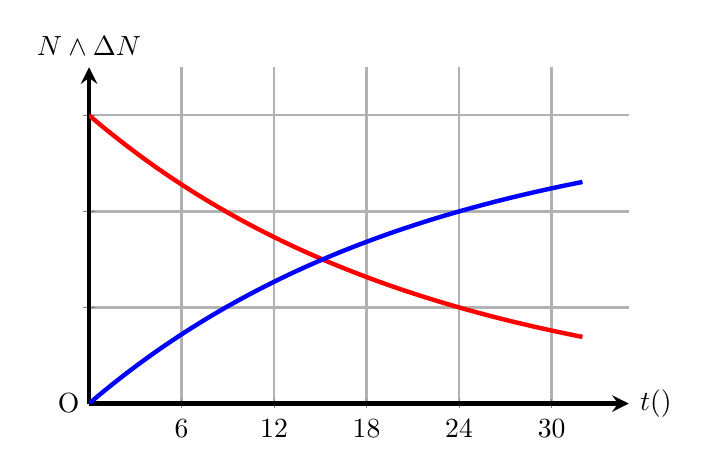
\begin{tikzpicture}  
			\begin{axis}[  ultra thick,yscale=0.75,
				xmin=0,  
				xmax=35,  
				xtick={0,6,...,30},
				ytick={0,1,2,3},
				yticklabels=\empty,
				minor x tick num=0,
				minor y tick num=0,
				ymin=0,  
				ymax=3.5, 
				samples=300,
				axis lines=center, 
				grid style={step=1, line width =0.4pt, color=gray!30!white},
				grid=both,
				major grid style={line width=0.8pt,gray!60!white},
				xlabel=$\xsi{t}{\left(\si{\hour}\right)}$, 		ylabel=$N\wedge\Delta N$,
				every axis y label/.style={at=(current axis.above origin),anchor=south},  
				every axis x label/.style={at=(current axis.right of origin),anchor=west},  ]
				\addplot [ultra thick, red, smooth, domain=0:32] {3*2^(-x/15.1423)};  
				\addplot [ultra thick, blue, smooth, domain=0:32] {3-3*2^(-x/15.1423)};
			\end{axis}  
			\node[left] at (0,0) {O};
		\end{tikzpicture}
		
	\end{center}
	\begin{enumerate}[label=\alph*)]
		\item Chu kì bán rã của X bằng bao nhiêu?
		\item Tại thời điểm $t=\SI{18}{\hour}$, số hạt X đã bị phân rã gấp mấy lần số hạt X còn lại trong mẫu?
	\end{enumerate}
	\loigiai{
	\begin{enumerate}[label=\alph*)]
		\item Dựa vào đồ thị, tại thời điểm $t=\SI{24}{\hour}$ thì
		$$\Delta N=2N\Leftrightarrow N_0\left(1-2^{-t/T}\right)=2N_0\cdot 2^{-t/T}\Leftrightarrow \left(1-2^{-\frac{24}{T}}\right)=2\cdot2^{-\frac{24}{T}}$$
		$\Rightarrow T\approx\SI{15.14}{\hour}.$
		\item Tại $t=\SI{18}{\hour}$:
		$$\dfrac{\Delta N}{N}=\dfrac{1-2^{-t/T}}{2^{-t/T}}=\dfrac{1-2^{-18/15,14}}{2^{-18/15,14}}\approx1,28.$$
		Vậy tại thời điểm $t=\SI{18}{\hour}$, số hạt X đã bị phân rã gấp 1,28 lần số hạt X còn lại.
	\end{enumerate}
	}
\end{vd}

\begin{dang}{Bài toán về số hạt nhân và khối lượng hạt nhân con tạo thành}
		Xét hạt nhân X phóng xạ ra tia phóng xạ C và biến đổi thành hạt nhân Y:
		\begin{equation}
			\ce{X}\longrightarrow \ce{Y}+\ce{C}
		\end{equation}
		Mỗi hạt nhân mẹ bị phân rã tạo thành một hạt nhân con nên số hạt nhân con tạo thành đúng bằng số hạt nhân mẹ bị phân rã:
		\begin{equation}
			\begin{cases}
				N_{\ce{Y}}=\Delta N_{\ce{X}}=N_{\ce{0X}}\left(1-2^{-t/T}\right)\\
				n_{\ce{Y}}=\Delta n_{\ce{X}}=n_{\ce{0X}}\left(1-2^{-t/T}\right)
			\end{cases}
		\end{equation}
		Khối lượng hạt nhân con Y được tạo thành sau thời gian $t$ là
		\begin{equation}
			n_{\ce{Y}}=n_{\ce{0X}}\left(1-2^{-t/T}\right)\Leftrightarrow \dfrac{m_{\ce{Y}}}{A_{\ce{Y}}}=\dfrac{m_0}{A_{\ce{X}}}\left(1-2^{-t/T}\right)\Rightarrow m_{\ce{Y}}=m_0\left(1-2^{-t/T}\right)\dfrac{A_{\ce{Y}}}{A_{\ce{X}}}
		\end{equation}
\end{dang}
\begin{vd}
	Chất polonium $\ce{^{210}_{84}Po}$ phóng xạ alpha $\left(\alpha\right)$ và chuyển thành chì $\ce{^{206}_{82}Pb}$ với chu kỳ bán rã là 138,4 ngày. Khối lượng ban đầu của $\ce{Po}$ là $\SI{50}{\gram}$.
	\begin{enumerate}[label=\alph*)]
		\item Sau 100 ngày (kể từ thời điểm ban đầu) thì tỉ số của số hạt nhân $\ce{Pb}$ và $\ce{Po}$ bằng bao nhiêu?
		\item Sau bao lâu khối lượng hạt nhân $\ce{Po}$ gấp 4 lần khối lượng hạt nhân $\ce{Pb}$?
	\end{enumerate}
	\loigiai{
	Phương trình phản ứng: $\ce{^{210}_{84}Po}\longrightarrow \ce{^4_2\alpha}+\ce{^{206}_{82}Pb}$.
	\begin{enumerate}[label=\alph*)]
		\item Sau 100 ngày (kể từ thời điểm ban đầu) thì tỉ số của số hạt nhân $\ce{Pb}$ và $\ce{Po}$ là
		$$\dfrac{N_{\ce{Pb}}}{N_{\ce{Po}}}=2^{t/T}-1=2^{\frac{100}{138,4}}-1\approx0,6524.$$
		\item Ta có:
		$$\dfrac{m_{\ce{Pb}}}{m_{\ce{Po}}}=\dfrac{A_{\ce{Pb}}}{A_{\ce{Po}}}\left(2^{t/T-1}\right)\Leftrightarrow \dfrac{1}{4}=\dfrac{206}{210}\left(2^{\frac{t}{138,4}}-1\right)\Rightarrow t=\SI{45.1977}{\text{ngày}}.$$
	\end{enumerate}	
	}
\end{vd}
	% ============================
	\begin{vd}
		Hạt nhân uranium $\ce{^{238}_{92}U}$ sau một chuỗi phân rã, biến đổi thành hạt nhân chì $\ce{^{206}_{82}Pb}$. Trong quá trình đó, chu kì bán rã của $\ce{^{238}_{92}U}$ biến đổi thành hạt nhân chì là $\SI{4.47E9}{\text{năm}}$. Một khối đá được phát hiện có chứa $\SI{1.188E20}{}$ hạt nhân $\ce{^{238}_{92}U}$ và $\SI{6.239E18}{}$ hạt nhân $\ce{^{206}_{82}Pb}$. Giả sử khối đá lúc mới hình thành không chứa hạt nhân chì và tất cả lượng hạt nhân chì có mặt trong đó đều là sản phẩm phân rã của $\ce{^{238}_{92}U}$. Tuổi của khối đá khi được phát hiện là bao nhiêu?
		\loigiai{
		Số hạt chì tạo thành bằng số hạt uranium đã phóng xạ: $N_{\ce{Pb}}	=\Delta N_{\ce{U}}$.\\
		Theo đề bài, ta có:
		$$\dfrac{N_{\ce{Pb}}}{N_{\ce{U}}}=\dfrac{\Delta N_{\ce{U}}}{N_{\ce{U}}}=\dfrac{N_0\left(1-2^{-t/T}\right)}{N_0\cdot2^{-t/T}}=2^{t/T}-1=\dfrac{\SI{6.239E18}{}}{\SI{1.188E20}{}}=0,0525.$$
		$$\Rightarrow2^{t/T}=1,0525\Rightarrow t=\SI{3.3E8}{\text{năm}}.$$
		Vậy tuổi của khối đá khi được phát hiện là $\SI{3.3E8}{\text{năm}}$.
		}
	\end{vd}
	\begin{dang}{Định nghĩa được độ phóng xạ, hằng số phóng xạ và vận dụng được mối liên hệ $H=\lambda N$}
	\end{dang}
	\begin{vd}
		Một mẫu chất phóng xạ $\beta^+$ là $\ce{^{15}_8O}$ có độ phóng xạ là $\SI{2.80E7}{\becquerel}$. Biết rằng hằng số phóng xạ của $\ce{^{15}_8O}$ là $\SI{5.67E-3}{\second^{-1}}$.
		\begin{enumerate}[label=\alph*)]
			\item Xác định số hạt nhân chất phóng xạ có trong mẫu khi đó.
			\item Xác định số hạt positron mẫu chất phát ra trong khoảng thời gian $\SI{1.00}{\milli\second}$. Coi gần đúng rằng độ phóng xạ của mẫu không thay đổi trong khoảng thời gian rất ngắn này.
		\end{enumerate}
		\loigiai{\begin{enumerate}[label=\alph*)]
				\item Số hạt nhân chất phóng xạ có trong mẫu khi đó:
				$$N_0=\dfrac{H_0}{\lambda}=\dfrac{\SI{2.80E7}{\becquerel}}{\SI{5.67E-3}{\second^{-1}}}\approx\SI{49.38E8}{\text{hạt}}.$$
				\item Trong quá trình phóng xạ trên diễn ra, mỗi hạt nhân bị phóng xạ sẽ phát ra một hạt positron. Do đó, số hạt positron mẫu chất phát ra bằng số hạt nhân $\ce{^{15}_8O}$ phân rã:
				$$N_{\beta^+}=\Delta N=N_0\left(1-e^{-\lambda t}\right)=\SI{49.38E8}{}\cdot\left[1-e^{-\left(\SI{5.67E-3}{\second^{-1}}\right)\cdot\left(\SI{1.00E-3}{\second}\right)}\right]\approx\SI{27998}{\text{hạt}}.$$
		\end{enumerate}}
	\end{vd}
% ===============================================
\begin{vd}
	Nhờ một máy đếm xung người ta có được thông tin sau về 1 chất phóng xạ. Ban đầu, trong thời gian 1 phút có 360 nguyên tử của chất phóng xạ, nhưng 2 giờ sau (kể từ thời điểm ban đầu) thì trong 1 phút chỉ có 90 nguyên tử phóng xạ. Tìm chu kì bán rã của chất phóng xạ này.
	\loigiai{
	Độ phóng xạ ban đầu: $H_0=\dfrac{360}{60}=\SI{6}{\becquerel}$.\\
	Độ phóng xạ sau 2 giờ: $H=\dfrac{90}{60}=\SI{1.5}{\becquerel}$.\\
	Từ $H=H_02^{-\frac{t}{T}}\Leftrightarrow 1,5=6\cdot 2^{-\dfrac{2}{T}}\Rightarrow T=\SI{1}{\hour}.$	
	}
\end{vd}
% ==================================
\begin{vd}
Một mẫu ban đầu chứa đồng vị $\ce{^{60}_{27}Co}$ nguyên chất, là chất phóng xạ $\gamma$ với chu kì bán rã $\SI{5.27}{\text{năm}}$ được sử dụng trong điều trị ung thư. Khi mẫu này được sử dụng lần đầu thì thời gian cho một liều chiếu xạ là 15 phút. Hỏi sau 2 năm, nếu vẫn sử dụng mẫu chất này thì thời gian cho một liều chiếu xạ là bao nhiêu? Coi như lượng hạt $\gamma$ cho một liều chiếu xạ trong cả hai lần là như nhau.
\loigiai{
Độ phóng xạ tại thời điểm ban đầu:
$$H_0=\dfrac{\Delta N_0}{\Delta t_0}$$
với $\Delta N_0$ là số hạt đã phân rã trong thời gian $\Delta t_0$.\\
Độ phóng xạ tại thời điểm $t$:
$$H=\dfrac{\Delta N}{\Delta t}$$
với $\Delta N$ là số hạt đã phân rã trong thời gian $\Delta t$.\\
Từ $H=H_0\cdot 2^{-\frac{t}{T}}\Rightarrow \dfrac{\Delta N}{\Delta t}=\dfrac{\Delta N_0}{\Delta t_0}\cdot 2^{-\frac{t}{T}}$.\\
Do liều chiếu xạ ở cả 2 lần là như nhau: $\Delta N_0=\Delta N\Rightarrow \Delta t=\Delta t_0\cdot 2^{\frac{t}{T}}=\left(\SI{15}{\minute}\right)\cdot2^{\frac{\SI{2}{\text{năm}}}{\SI{5.27}{\text{năm}}}}\approx\SI{19.5}{\minute}.$
}
\end{vd}
\subsection{Bài tập}
\subsubsection{Trắc nghiệm nhiều phương án lựa chọn}
\setcounter{ex}{0}
\Opensolutionfile{ans}[ans/VN12-Y24-PH-SYL-029P-TN]
% ===================================================================
\begin{ex}
	Chỉ ra phát biểu \textbf{sai} khi nói về hiện tượng phóng xạ.
	\choice
	{Hiện tượng phóng xạ là hiện tượng một hạt nhân không bền vững tự phát phân rã, phát ra các tia phóng xạ và biến đổi thành hạt nhân khác}
	{\True Hiện tượng phóng xạ chịu ảnh hưởng bởi các yếu tố bên ngoài như nhiệt độ, áp suất, $\dots$}
	{Có 3 loại phóng xạ là phóng xạ $\alpha, \beta$ và $\gamma$; trong đó phóng xạ $\beta$ được chia làm hai loại là phóng xạ $\beta^-$ và phóng xạ $\beta^{+}$}
	{Do tia $\gamma$ có bản chất là sóng điện từ nên phóng xạ $\gamma$ không đi kèm với việc biến đổi hạt nhân mẹ thành hạt nhân khác}
	\loigiai{
		
	}
\end{ex}
% ===================================================================
\begin{ex}
	Trong các định luật bảo toàn sau:
	\begin{enumerate}[label=(\arabic*)]
		\item Bảo toàn động lượng.
		\item Bảo toàn số khối.
		\item Bảo toàn khối lượng.
		\item Bảo toàn năng lượng toàn phần.
		\item Bảo toàn số proton.
	\end{enumerate}
	Hiện tượng phóng xạ tuân theo bao nhiêu định luật bảo toàn?
	\choice
	{2}
	{\True 3}
	{4}
	{5}
	\loigiai{
		Chọn (1); (2); (4).
	}
\end{ex}
% ===================================================================
\begin{ex}
	Tìm phát biểu \textbf{sai}.
	\choice
	{Hạt $\beta^{-}$ là hạt electron}
	{Tia $\beta^{-}$ có khả năng ion hoá môi trường}
	{Trong điện trường giữa hai bản tụ điện, tia $\beta^{-}$bị lệch về phía bản mang điện dương của tụ điện}
	{\True Tia $\beta^{-}$có tầm bay ngắn hơn tia $\alpha$}
	\loigiai{}
\end{ex}
% ===================================================================
\begin{ex}
	Tìm phát biểu \textbf{sai}.
	\choice
	{Tia $\beta^{+}$có tầm bay xa hơn tia $\alpha$}
	{Hạt $\beta^{+}$có cùng khối lượng với electron nhưng mang điện tích nguyên tố dương}
	{Tia $\beta^{+}$ cũng làm ion hoá môi trường nhưng yếu hơn tia $\alpha$}
	{\True Tia $\beta^{+}$ bị lệch về phía bản mang điện dương của tụ điện khi đi qua điện trường giữa hai bản tụ điện}
	\loigiai{}
\end{ex}
% ===================================================================
\begin{ex}
	Công thức nào dưới đây \textbf{đúng} với nội dung của định luật phóng xạ?
	\choice
	{$m=m_0e^{\lambda t}$}
	{\True $m=m_0e^{-\lambda t}$}
	{$m=m_0 e^{-\frac{\lambda}{t}}$}
	{$m=m_0 e^{-\frac{1}{T}}$}
	\loigiai{}
\end{ex}
% ===================================================================
\begin{ex}
	Trong một mẫu chất phóng xạ, tại thời điểm ban đầu $(t=0)$, mẫu chất có $N_0$ hạt nhân. Biết hằng số phóng xạ và chu kì bán rã của chất phóng xạ này lần lượt là $\lambda$ và $T$. Sau đó một khoảng thời gian $\Delta t$, số lượng hạt nhân còn lại trong mẫu chất đó được xác định bằng biểu thức nào sau đây?
	\choice
	{$N_{t}=N_0 e^{\lambda \Delta t}$}
	{$N_{t}=N_0 2^{\frac{\Delta t}{T}}$}
	{\True $N_{t}=N_0 e^{-2 \Delta t}$}
	{$N_{t}=N_0 2^{-\Delta t}$}
	\loigiai{}
\end{ex}
% ===================================================================
\begin{ex}
	Phát biểu nào sau đây là \textbf{sai} khi nói về độ phóng xạ?
	\choice
	{Độ phóng xạ là đại lượng đặc trưng cho tính phóng xạ mạnh hay yếu của một lượng chất phóng xạ}
	{Đơn vị đo độ phóng xạ là becquerel}
	{Với mỗi lượng chất phóng xạ xác định thì độ phóng xạ tỉ lệ với số nguyên tử của lượng chất đó}
	{\True Độ phóng xạ của một lượng chất phóng xạ phụ thuộc nhiệt độ của lượng chất đó}
	\loigiai{}
\end{ex}
% ===================================================================
\begin{ex}
	Trong các phát biểu sau khi nói về hiện tượng phóng xạ, có bao nhiêu phát biểu \textbf{đúng}?
	\begin{enumerate}[label=(\arabic*)]
		\item Chu kì bán rã là thời gian để một nửa số hạt nhân ban đầu bị phân rã.
		\item Mối quan hệ giữa chu kì bán rã và hằng số phóng xạ là $\lambda=T \cdot \ln 2$.
		\item Trong hiện tương phóng xạ, tia $\gamma$ thường sẽ phát kèm theo các tia $\alpha$ và $\beta$.
		\item Độ phóng xạ là đại lượng đặc trưng cho tính phóng xạ mạnh hay yếu của một lượng chất phóng xạ.
		\item Trong hiện tượng phóng xạ, độ phóng xạ tăng dần theo thời gian với quy luật hàm số mũ.
	\end{enumerate}
	\choice
	{1}
	{2}
	{\True 3}
	{4}
	\loigiai{Chọn phát biểu: 1; 3 và 4.}
\end{ex}
% ===================================================================
\begin{ex}
	Chiếu 3 chùm tia thu được từ quá trình phóng xạ hạt nhân lần lượt qua tấm giấy, nhôm và chì như hình bên. Các tia 1, tia 2, tia 3 theo thứ lần lượt là
	\begin{center}
		\includegraphics[width=0.4\linewidth]{figs/VN12-Y24-PH-SYL-031P-2}
	\end{center}
	\choice
	{tia $\beta$, tia $\alpha$, tia $\gamma$}
	{\True tia $\alpha$, tia $\beta$, tia $\gamma$}
	{tia $\beta$, tia $\gamma$, tia $\alpha$}
	{tia $\gamma$, tia $\alpha$, tia $\beta$}
	\loigiai{}
\end{ex}
% ===================================================================
\begin{ex}
	Bắn chùm tia phóng xạ qua không gian có từ trường đều như hình vẽ. Chùm tia A là 	
	\begin{center}
		\includegraphics[width=0.2\linewidth]{figs/VN12-Y24-PH-SYL-031P-1}
	\end{center}
	\choice
	{\True tia $\gamma$}
	{tia $\alpha$}
	{tia $\beta^+$}
	{tia $\beta^-$}
	\loigiai{
		Chùm gamma không mang điện tích nên không bị lệch phương trong từ trường.	
	}
\end{ex}
% ===================================================================
\begin{ex}
	Bắn chùm tia phóng xạ qua không gian có từ trường đều như hình vẽ. Chùm tia C là 	
	\begin{center}
		\includegraphics[width=0.2\linewidth]{figs/VN12-Y24-PH-SYL-031P-1}
	\end{center}
	\choice
	{tia $\gamma$}
	{tia $\alpha$}
	{tia $\beta^+$}
	{\True tia $\beta^-$}
	\loigiai{
		Chùm tia $\beta^-$ mang là chùm $e^-$ mang điện tích âm, áp dụng quy tắc bàn tay trái, lực từ tác dụng lên $e^-$ làm nó lệch hướng cùng chiều quay của kim đồng hồ.
	}
\end{ex}
% ===================================================================
\begin{ex}
	Chùm tia $\alpha$ và $\beta^-$ được bắn ra với cùng động năng phi tương đối tính. Tỉ số giữa mỗi hạt trong 2 chùm tia là
	\choice
	{\True $\dfrac{v_\beta}{v_\alpha}=85,73$}
	{$\dfrac{v_\beta}{v_\alpha}=2$}
	{$\dfrac{v_\beta}{v_\alpha}=60,6$}
	{$\dfrac{v_\beta}{v_\alpha}=4$}
	\loigiai{
		$$K_\alpha=K_\beta\Leftrightarrow \dfrac{1}{2}m_\alpha v^2_\alpha=\dfrac{1}{2}m_\beta v^2_\beta$$
		$$\Rightarrow \dfrac{v_\beta}{v_\alpha}=\sqrt{\dfrac{m_\alpha}{m_\beta}}=\sqrt{\dfrac{4m_p}{m_e}}\approx 85,7.$$
	}
\end{ex}
% ===================================================================
\begin{ex}
	Hình bên dưới là mặt đồng hồ của máy bay thế chiến II phát sáng trong bóng tối, vì chúng được sơn bằng sơn phát quang pha radium (có chu kì bán rã 1602 năm). Mặc dù mặt đồng hồ sơn radium có thể nhìn thấy dễ dàng cả ngày lẫn đêm, nhưng chúng phát ra radon, một loại khí phóng xạ nguy hiểm và không thể cảm nhận trực tiếp. 
	\begin{center}
		\includegraphics[width=0.4\linewidth]{figs/VN12-Y24-PH-SYL-032P-1}
		\captionof{figure}{Mặt đồng hồ trong máy bay được sơn bằng sơn phát quang có pha radium.}
	\end{center}
	Nếu độ phóng xạ ban đầu của radium khi mới được sơn là $\SI{E5}{\becquerel}$ thì độ phóng xạ còn lại sau 57 năm kể từ khi sản xuất là
	\choice
	{$\SI{96504.5}{\becquerel}$}
	{$\SI{2436.1}{\becquerel}$}
	{\True $\SI{97563.9}{\becquerel}$}
	{$\SI{3495.5}{\becquerel}$}
	\loigiai{
		Độ phóng xạ còn lại:
		$$H=H_0\cdot 2^{-\dfrac{t}{T}}=\left(\SI{E5}{\becquerel}\right)\cdot 2^{-\dfrac{57}{1602}}\approx\SI{97563.9}{\becquerel}.$$
	}
\end{ex}
% ===================================================================
\begin{ex}
	Hiện nay đồng vị phóng xạ $\ce{_9^{18}F}$ được sử dụng rộng rãi trong việc chẩn đoán các bệnh ung thư nhờ vào công nghệ chụp cắt lớp bằng phát xạ positron (Positron Emission Tomography - PET). Giả sử rằng một bệnh nhân được tiêm một lượng chất phóng xạ $\ce{_9^{18}F}$ với độ phóng xạ là $\SI{350}{\becquerel}$ trước khi quá trình chụp ảnh diễn ra. Hỏi sau bao lâu kể từ thời điểm tiêm thì độ phóng xạ trong cơ thể bệnh nhân giảm còn $\SI{25}{\becquerel}$? Biết rằng chu kì bán rã của $\ce{_9^{18}F}$ là 110 ngày.
	\choice
	{378,92 ngày}
	{427,93 ngày}
	{\True 418,81 ngày}
	{125,46 ngày}
	\loigiai{
		Khoảng thời gian cần tìm là:
		$$H_t=H_02^{-\dfrac{t}{T}}\Rightarrow 25=350\cdot 2^{-\frac{t}{110}}\Rightarrow t\approx\SI{418.81}{\text{ngày}}.$$
	}
\end{ex}
% ===================================================================
\begin{ex}
	Một mẫu phóng xạ có chu kì bán rã là 3 ngày. Sau 9 ngày, khối lượng của mẫu phóng xạ này còn lại là $\SI{2}{\kilogram}$. Khối lượng ban đầu của mẫu là bao nhiêu?
	\choice
	{$\SI{15}{\kilogram}$}
	{\True $\SI{16}{\kilogram}$}
	{$\SI{17}{\kilogram}$}
	{$\SI{14}{\kilogram}$}
	\loigiai{
		
	}
\end{ex}
% ===================================================================
\begin{ex}
	$\ce{_{84}^{210}Po}$ là một đồng vị phóng xạ có chu kì bán rã là 138,4 ngày. Xét một mẫu chất đang chứa $N_0$ hạt nhân $\ce{_{84}^{210}Po}$ (tại thời điểm ban đầu). Sau bao lâu kể từ thời điểm ban đầu thì tỉ số giữa số hạt nhân $\ce{_{84}^{210}Po}$ đã phân rã thành hạt nhân khác và số hạt nhân $\ce{_{84}^{210}Po}$ còn lại bằng 7 ?
	\choice
	{\True 415,2 ngày}
	{387,5 ngày}
	{34,6 ngày}
	{968,8 ngày}
	\loigiai{Khoảng thời gian cần tìm là:
		$$
		\frac{\Delta N_{t}}{N_{t}}=\frac{N_0\left(1-2^{-\frac{t}{T}}\right)}{N_0 2^{-\frac{t}{T}}}=2^{\frac{t}{T}}-1=7 \Rightarrow t=3 T=3\cdot138,4=\SI{415.2}{\text{ngày}}.
		$$}
\end{ex}
% ===================================================================
\begin{ex}
	Chu kì bán rã của một mẫu phóng xạ là 6 giờ. Lúc đầu mẫu có khối lượng $\SI{2.4E-2}{\kilogram}$. Hỏi sau một ngày đêm, khối lượng của mẫu còn lại bằng bao nhiêu?
	\choice
	{$\SI{3E-3}{\kilogram}$}
	{\True $\SI{1.5E-3}{\kilogram}$}
	{$\SI{2.5E-3}{\kilogram}$}
	{$\SI{2E-3}{\kilogram}$}
	\loigiai{}
\end{ex}
% ===================================================================
\begin{ex}
	Sau 3 giờ phóng xạ, số hạt nhân của một mẫu đồng vị phóng xạ chỉ còn $\SI{25}{\percent}$ số hạt nhân ban đầu. Chu kì bán rã của đồng vị này là
	\choice
	{1 giờ}
	{2 giờ}
	{2,5 giờ}
	{\True 1,5 giờ}
	\loigiai{}
\end{ex}
% ===================================================================
\begin{ex}
	Một mẫu chất phóng xạ $X$ phân rã theo thời gian và phát ra các hạt $\alpha$. Số lượng các hạt $\alpha$ này được ghi nhận bởi một máy thu (ống Geiger-Muller) và được biểu diễn theo thời gian $t$ như đồ thị ở hình bên.
	\begin{center}
		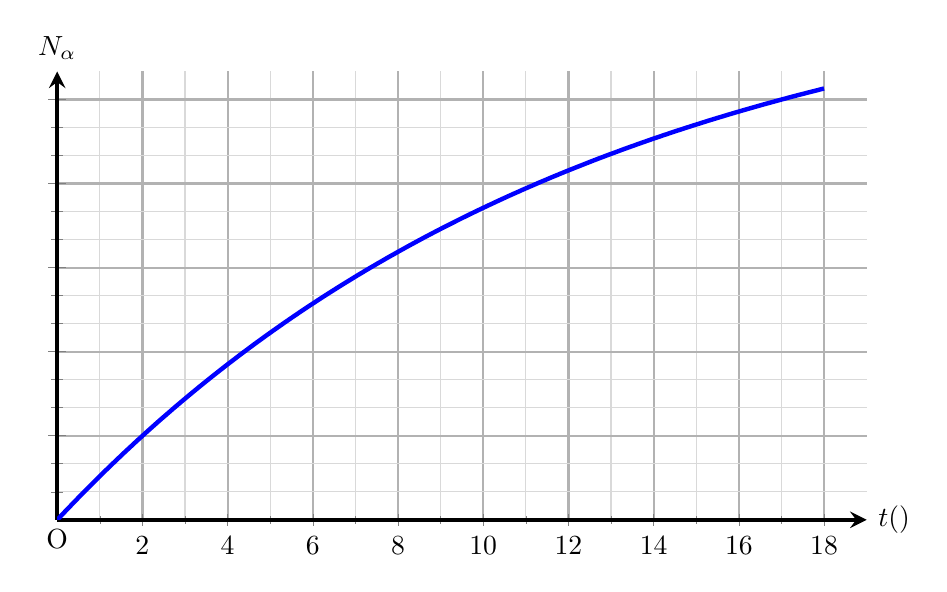
\begin{tikzpicture}  
			\begin{axis}[  ultra thick,
				xmin=0,  
				xmax=19,  
				xtick={0,2,...,18},
				ytick={0,3,...,15},
				minor x tick num=1,
				minor y tick num=2,
				ymin=0,  
				ymax=16, 
				samples=300,
				yticklabels=\empty,
				axis lines=center, 
				grid style={step=1, line width =0.4pt, color=gray!30!white},
				grid=both, %giới hạn ô lưới
				major grid style={line width=0.8pt,gray!60!white},
				xlabel=$\xsi{t}{\left(\si{\second}\right)}$, 		ylabel=$N_{\alpha}$,
				every axis y label/.style={at=(current axis.above origin),anchor=south},  
				every axis x label/.style={at=(current axis.right of origin),anchor=west}, xscale=1.5 ]
				\addplot [ultra thick, blue, smooth, domain=0:18] {20.0647*(1-2^(-x/8.56))};  
			\end{axis}  
			\node[below] at (0,0) {O};
		\end{tikzpicture}
	\end{center}
	Hằng số phóng xạ của chất phóng xạ là
	\choice
	{\True $\SI{0.081}{\second^{-1}}$}
	{$\SI{0.173}{\second^{-1}}$}
	{$\SI{0.231}{\second^{-1}}$}
	{$\SI{0.058}{\second^{-1}}$}
	\loigiai{
		$$
		\begin{aligned}
			& N_\alpha=N_0 \cdot\left(1-2^{-\frac{t}{T}}\right) \Rightarrow
			\begin{cases}
				3=N_0 \cdot\left(1-2^{-\frac{2}{T}}\right) \\
				15=N_0 \cdot\left(1-2^{-\frac{17}{T}}\right)
			\end{cases}
			\Rightarrow \frac{3}{15}=\frac{1-2^{-\frac{2}{T}}}{1-2^{-\frac{17}{T}}} \Rightarrow T \approx \SI{8.56}{\second} \\
			& \Rightarrow \lambda=\frac{\ln 2}{T}=\frac{\ln 2}{8,56} \approx \SI{0.081}{\second^{-1}}.
		\end{aligned}
		$$
	}
\end{ex}
% ===================================================================
\begin{ex}
	Nguồn polonium $\left(\ce{^{210}Po}\right)$ được sử dụng trong phòng thí nghiệm vật lý có độ phóng xạ $\SI{1.0}{\micro Ci}$ vào ngày chuẩn bị mẫu. Sau 120 ngày, một sinh viên vào phòng thí nghiệm đo độ phóng xạ của nguồn bằng máy đếm Geiger và thu được 1500 lần đếm mỗi phút. Biết chu kì bán rã của polonium là 138 ngày. Trong thí nghiệm trên, máy đã ghi nhận được bao nhiêu phần trăm phân rã do nguồn phát ra?
	\choice
	{$\SI{12.3}{\percent}$}
	{$\SI{0.74}{\percent}$}
	{$\SI{7.4}{\percent}$}
	{\True $\SI{0.123}{\percent}$}
	\loigiai{
		Độ phóng xạ còn lại sau 120 ngày:
		$$H=H_0\cdot2^{-\dfrac{t}{T}}=\left(\SI{E-6}{Ci}\right)\cdot\left(\SI{3.7E10}{\becquerel/Ci}\right)\cdot 2^{-\dfrac{120}{138}}=\SI{20250.5}{\becquerel}.$$
		Số phân rã trong 1 phút sau 120 ngày:
		$$\Delta N=H\Delta t=\left(\SI{20250.5}{\becquerel}\right)\cdot\left(\SI{60}{\second}\right)=\SI{1215032}{\text{phân rã}}.$$
		Tỉ lệ phân rã được máy ghi nhận:
		$$\dfrac{\Delta N'}{\Delta N}\cdot\SI{100}{\percent}=\dfrac{1500}{1215032}\cdot\SI{100}{\percent}\approx\SI{0.123}{\percent}.$$
	}
\end{ex}
% ===================================================================
\begin{ex}
	Trong khảo cổ học để đánh giá tuổi của các vật liệu hữu cơ như gỗ và da, người ta thường sử dụng kỹ thuật xác định tuổi bằng carbon phóng xạ. Cơ sở của kĩ thuật này là mật độ  nguyên tử $\ce{^{14}C}$ trong khí quyển gần như không đổi và có giá trị bằng $1,3$ nguyên tử $\ce{^{14}C}$ trong mỗi $10^{12}$ nguyên tử carbon bao gồm tất cả các đồng vị. Tuy nhiên, khi một cơ thể sống chết đi, $\ce{^{14}C}$ không còn được cung cấp nữa và bắt đầu giảm đi phóng xạ $\beta$ với thời gian bán rã $\SI{5730}{\text{năm}}$:
	$$\ce{^{14}_6C}\longrightarrow \ce{^{14}_7N}+e^{-}+\overline{\nu}_e$$
	Giả sử có $\SI{50}{\gram}$ carbon từ một mảnh gỗ tìm được trong một ngôi mộ tiền sử. Biết khối lượng nguyên tử trung bình của carbon là $\SI{2e-26}{\kilogram}$. Người ta không thể đếm trực tiếp số nguyên tử $\ce{^{14}C}$ được nhưng có thể đếm được tổng số $935$ electron phát xạ từ mảnh gỗ trên trong 10 phút. Tuổi của ngôi mộ là
	\choice
	{19359 năm}
	{\True 17190 năm}
	{13223 năm}
	{15021 năm}
	\loigiai{
		Số nguyên tử $\ce{^{14}C}$ ban đầu trong mảnh gỗ:
		$$N_0=\dfrac{m}{m_0}\cdot\dfrac{1,3}{10^12}=\SI{3.25E12}{}.$$
		Độ phóng xạ của mẫu gỗ ở thời điểm phát hiện:
		$$H=\dfrac{\Delta N}{\Delta t}=\lambda N_0e^{-\lambda T}$$
		Tuổi của mẫu vật:
		$$\begin{aligned}
			&t=-\dfrac{1}{\lambda}\cdot\ln\left(\dfrac{1}{\lambda N_0}\cdot\dfrac{\Delta N}{\Delta t}\right)=-\dfrac{T}{\ln2}\cdot\ln\left(\dfrac{T}{N_0\ln 2}\cdot\dfrac{\Delta N}{\Delta t}\right)\\
			\Rightarrow &t=-\dfrac{\left(\SI{5730}{\text{năm}}\right)}{\ln2}\cdot\ln\left(\dfrac{5730\cdot365\cdot24\cdot\SI{60}{\minute}}{\SI{3.25E12}{}\cdot\ln2}\cdot\dfrac{935}{\SI{10}{\minute}}\right)\approx\SI{17190}{\text{năm}}.
		\end{aligned}
		$$}
\end{ex}

% ===================================================================
\begin{ex}
	Tỉ lệ uranium hiện tại trong tự nhiên là $\SI{0.72}{\percent}\ \ce{^{235}U}$ và $\SI{99.27}{\percent}\ \ce{^{238}U}$. Tỉ lệ phần trăm của $\ce{^{235}U}$ trong tự nhiên sẽ là bao nhiêu nếu ở thời điểm Trái Đất được hình thành (cách nay 4,5 tỉ năm)? Biết rằng chu kì bán rã của $\ce{^{235}U}$ là 704 triệu năm và của $\cee{^{238}U}$ là 4,47 tỉ năm.
	\choice
	{$\SI{26.73}{\percent}$}
	{\True $\SI{23.26}{\percent}$}
	{$\SI{99.98}{\percent}$}
	{$\SI{98.56}{\percent}$}
	\loigiai{
		Gọi $a$ là tỉ lệ phần trăm $\ce{^{235}U}$ ban đầu trong tự nhiên và $N_0$ là tổng số hạt uranium khi Trái Đất mới hình thành.
		\begin{center}
			\begin{tabular}{|C{4cm}|C{5cm}|C{5cm}|}
				\hline
				\textbf{Đồng vị}&\textbf{Ban đầu}& \textbf{Hiện tại}\\
				\hline
				$\ce{^{235}U}$ & $a\cdot N_0$ & $a\cdot N_0\cdot 2^{-\dfrac{t}{T_{235}}}$\\
				\hline
				$\ce{^{238}U}$ & $\left(1-a\right)\cdot N_0$ & $\left(1-a\right)\cdot N_0\cdot 2^{-\dfrac{t}{T_{238}}}$\\
				\hline
			\end{tabular}
		\end{center}	
		Ta có:
		$$\si{\percent}\ce{^{235}U}=\dfrac{N_{\ce{^{235}U}}}{N_{\ce{^{235}U}+N_{\ce{^{238}U} }}}=\dfrac{a\cdot2^{-\dfrac{t}{T_{235}}}}{a\cdot2^{-\dfrac{t}{T_{235}}}+\left(1-a\right)\cdot2^{-\dfrac{t}{T_{238}}}}$$
		$$\Leftrightarrow\SI{0.72}{\percent}=\dfrac{a\cdot2^{-\dfrac{4,5}{\SI{704E-3}{}}}}{a\cdot2^{-\dfrac{4,5}{\SI{704E-3}{}}}+\left(1-a\right)\cdot2^{-\dfrac{4,5}{4,47}}}\Rightarrow a=\SI{23.26}{\percent}.$$
	}
\end{ex}
\Closesolutionfile{ans}
\subsubsection{Trắc nghiệm đúng/sai}
\Opensolutionfile{ans}[ans/VN12-Y24-PH-SYL-029P-TF]
\setcounter{ex}{0}
% ===================================================================
\begin{ex}
	Nhận định các phát biểu sau:
	\choiceTF[t]
	{Phân rã phóng xạ cần có kích thích để xảy ra}
	{\True Tia phóng xạ là tia không nhìn thấy được, nhưng có các tính chất như: ion hóa, gây ra các hiệu ứng quang điện, phát xạ thứ cấp, làm đen kính ảnh, xuyên thấu lớp vật chất mỏng, phá hủy tế bào, kích thích một số phản ứng hóa học, \dots}
	{Tia phóng xạ $\gamma$ là chùm hạt mang điện dương và có khả năng đâm xuyên rất lớn}
	{\True Nguyên tắc an toàn khi làm việc với nguồn phóng xạ: giữ khoảng cách đủ xa đối với nguồn phóng xạ, cần sử dụng các tấm chắn nguồn phóng xạ đủ tốt và cần giảm thiểu thời gian phơi nhiễm phóng xạ}
	\loigiai{}
\end{ex}
% ===================================================================
\begin{ex}
	$\ce{_{92}^{238}U}$ là một đồng vị phóng xạ có hằng số phóng xạ bằng $\SI{4.916E-18}{\second^{-1}}$. Biết rằng sau một khoảng thời gian nào đó, $\ce{_{92}^{238}U}$ xảy ra phóng xạ $\alpha$ và biến đổi thành hạt nhân con $\ce{X }$. Trong mỗi phát biểu sau, em hãy chọn đúng hoặc sai.
	\choiceTF[t]
	{\True Quá trình phóng xạ của $\ce{_{92}^{238}U}$ là một phản ứng hạt nhân toả năng lượng}
	{Hạt nhân con $\ce{X}$ được tạo thành từ quá trình phóng xạ trên là $\ce{_{92}^{234}U}$}
	{\True Chu kì bán rã của $\ce{_{92}^{238}U}$ là $\SI{1.41E17}{\second}$ (làm tròn đến 2 chữ số thập phân sau dấu phẩy)}
	{Xét một mẫu chất tại thời điểm ban đầu chứa $\SI{0.1}{\gram}$ đồng vị phóng xạ $\ce{_{92}^{238}U}$. Sau 100 triệu năm (xem như mỗi năm có 365 ngày), khối lượng $\ce{_{92}^{238}U}$ còn lại trong mẫu chất đó khoảng $\SI{0.089}{\gram}$}
	\loigiai{}
\end{ex}
% ===================================================================
\begin{ex}
	Máy chiếu xạ sử dụng nguồn phóng xạ $\beta^{-}$ cobalt $\ce{_{27}^{60}Co}$ với chu kì bán rã 5,27 năm để điều trị ung thư. Nguồn phóng xạ trong máy sẽ cần được thay mới nếu như độ phóng xạ của nó giảm còn bằng $\SI{50}{\percent}$ độ phóng xạ ban đầu. Các phát biểu dưới đây là đúng hay sai?
	\choiceTF[t]
	{Sản phẩm phân rã của cobalt $\ce{_{27}^{60}Co}$ là nickel $\ce{_{28}^{61}Ni}$}
	{Hằng số phóng xạ của cobalt $\ce{_{27}^{60}Co}$ là $\SI{0.132}{\second^{-1}}$}
	{\True Nguồn phóng xạ của máy cần được thay thế sau mỗi 5,27 năm}
	{\True Tại thời điểm thay nguồn phóng xạ, số hạt nhân $\ce{_{27}^{60}Co}$ còn lại trong nguồn bằng $\SI{50}{\percent}$ số hạt nhân $\ce{_{27}^{60}Co}$ ban đầu}
	\loigiai{}
\end{ex}
% ===================================================================
\begin{ex}
	Radon $\left(\ce{^{222}Rn}\right)$ là khí phóng xạ không màu, không mùi, có chu kì bán rã 3,8 ngày. Radon được tạo thành do sự phân rã của uranium, radium, \dots trong đất và đá. Do sự chênh lệch áp suất, radon dễ dàng đi vào trong nhà thông qua các vết nứt, sàn nhà. 
	\begin{center}
		\includegraphics[width=0.4\linewidth]{figs/VN12-Y24-PH-SYL-032P-2}
		\captionof{figure}{Radon theo các vết nứt trên sàn vào trong nhà.}
	\end{center}
	Radon là chất gây ung thư phổi chỉ sau thuốc lá. Khi được hít vào phổi, radon tích tụ trong phổi và phóng xạ alpha gây tổn thương các mô phổi. Do đó, Cơ quan Bảo vệ Môi trường Hoa Kỳ (EPA) khuyến cáo rằng bất kỳ nhà hoặc văn phòng nào đo trên mức $\SI{4.0}{\pico Ci/\liter}$ cần phải được khắc phục ngay lập tức.
	
	\choiceTF[t]
	{Nếu áp suất trong nhà cao hơn áp suất trong đất, radon dễ dàng vào trong nhà hơn}
	{\True Phương trình phân rã của radon là $\ce{^{222}_{86}Rn}\longrightarrow \ce{^{218}_{84}Po}+\ce{^4_2He}$}
	{Ở các nước ôn đới, chu kì bán rã của radon dài hơn do nhiệt độ thấp}
	{\True Với mức khuyên cáo của EPA ($\SI{4.0}{\pico Ci/\liter}$), một căn nhà kích thước $\SI{5}{\meter}\times \SI{10}{\meter}\times \SI{4}{\meter}$ sẽ có khoảng 14 tỉ nguyên tử radon trong không khí}
	\loigiai{
		\begin{itemchoice}
			\itemch Sai. Nếu áp suất trong nhà thấp hơn áp suất trong đất, radon dễ dàng vào nhà hơn.
			\itemch Đúng. Phương trình thoả bảo toàn số khối và bảo toàn điện tích.
			\itemch Sai. Quá trình phóng xạ không phụ thuộc điều kiện bên ngoài.
			\itemch Đúng. Với độ phóng xạ $h=\SI{4.0}{\pico Ci/\liter}$ thì khối lượng radon trong căn phòng là
			$$\begin{aligned}
				&N=\dfrac{H}{\lambda}=\dfrac{hV}{\lambda}\\
				\Rightarrow & N=\dfrac{\left(\SI{4.0E-9}{Ci/\meter^3}\right)\cdot\left(\SI{3.7E10}{\becquerel/Ci}\right)\cdot\left(\SI{200}{\meter^3}\right)}{\dfrac{\ln 2}{3,8\cdot 24\cdot\SI{3600}{\second}}}\approx\SI{14E9}{\text{hạt}}.
			\end{aligned}$$
		\end{itemchoice}
	}
\end{ex}
% ===================================================================
\begin{ex}
	Hình bên biểu diễn sự phụ thuộc của số hạt còn lại và số hạt đã bị phân rã theo thời gian $t$ của một mẫu chất phóng xạ.
	\begin{center}
		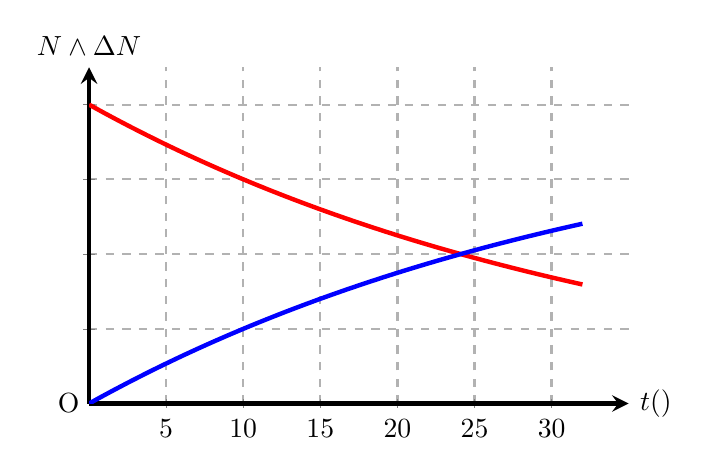
\begin{tikzpicture}  
			\begin{axis}[  ultra thick,yscale=0.75,
				xmin=0,  
				xmax=35,  
				xtick={0,5,...,30},
				ytick={0,1,...,5},
				yticklabels=\empty,
				minor x tick num=0,
				minor y tick num=0,
				ymin=0,  
				ymax=4.5, 
				samples=300,
				axis lines=middle, 
				grid style={step=1, line width =0.4pt, color=gray!30!white},
				grid=both,
				major grid style={line width=0.8pt,gray!60!white, dashed},
				xlabel=$\xsi{t}{\left(\si{\hour}\right)}$, 		ylabel=$N\wedge\Delta N$,
				every axis y label/.style={at=(current axis.above origin),anchor=south},  
				every axis x label/.style={at=(current axis.right of origin),anchor=west},  ]
				\addplot [ultra thick, red, smooth, domain=0:32] {4*2^(-x/24.094)};  
				\addplot [ultra thick, blue, smooth, domain=0:32] {4-4*2^(-x/24.094)};
			\end{axis}  
			
			\node[left] at (0,0) {O};
		\end{tikzpicture}
		
	\end{center}	
	\choiceTF[t]
	{Tại thời điểm $\SI{10}{\hour}$, số hạt bị phân rã gấp 3 lần số hạt còn lại}
	{Chu kì bán rã của mẫu chất là $\SI{25}{\hour}$}
	{\True Tại thời điểm $\SI{30}{\hour}$, số hạt nhân phóng xạ đã giảm 2,37 lần so với ban đầu}
	{Nếu tăng áp suất trong phóng, quá trình phòng xạ của mẫu chất sẽ diễn ra nhanh hơn}
	\loigiai{
		\begin{itemchoice}
			\itemch Sai. Tại thời điểm $\SI{10}{\hour}$, số hạt còn lại gấp 3 lần số hạt bị phân rã.
			\itemch Sai. Chu kì bán rã của mẫu chất là $T\approx\SI{24.09}{\hour}$.\\
			Tại thời điểm $t=\SI{10}{\hour}$ thì $N=\dfrac{3}{4}N_0$ nên:
			$$2^{-\dfrac{10}{T}}=\dfrac{3}{4}\Rightarrow T\approx\SI{24.09}{\hour}.$$
			\itemch Đúng. Tại thời điểm $t=\SI{30}{\hour}$ thì số hạt còn lại
			$$N=\dfrac{N_0}{2^{\dfrac{t}{T}}}=\dfrac{N_0}{2^{\dfrac{30}{24,09}}}\approx\dfrac{N_0}{2,37}.$$
			\itemch Sai. Quá trình phóng xạ không phụ thuộc điều kiện bên ngoài.
		\end{itemchoice}	
	}
\end{ex}
% ===================================================================
\begin{ex}
	Hai mẫu chất phóng xạ X và Y với chu kì bán rã có đồ thị biểu diễn số hạt phụ thuộc theo thời gian như hình bên. Nhận định các phát biểu sau đây:
	\begin{center}
		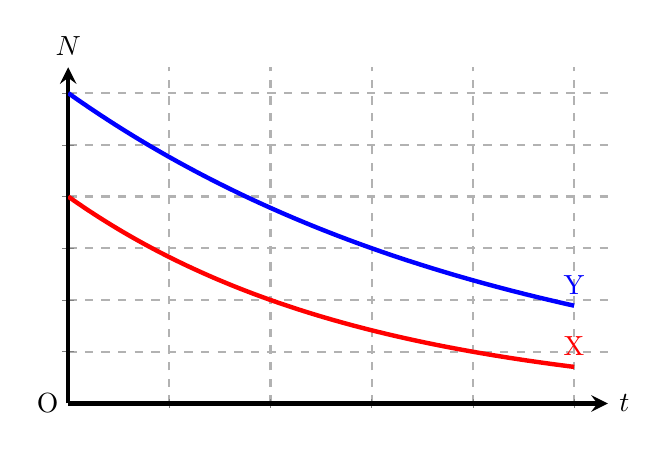
\begin{tikzpicture}  
			\begin{axis}[  ultra thick,yscale=0.75,
				xmin=0,  
				xmax=16,  
				xtick={0,3,...,15},
				ytick={0,1,...,6},
				yticklabels=\empty,
				xticklabels=\empty,
				minor x tick num=0,
				minor y tick num=0,
				ymin=0,  
				ymax=6.5, 
				samples=300,
				axis lines=middle, 
				grid style={step=1, line width =0.4pt, color=gray!30!white},
				grid=both,
				major grid style={line width=0.8pt,gray!60!white, dashed},
				xlabel=$t$, 		ylabel=$N$,
				every axis y label/.style={at=(current axis.above origin),anchor=south},  
				every axis x label/.style={at=(current axis.right of origin),anchor=west},  ]
				\addplot [ultra thick, red, smooth, domain=0:15] {4*2^(-x/6)} node [above] {X};  
				\addplot [ultra thick, blue, smooth, domain=0:15] {6*2^(-x/9)} node [above] {Y};
			\end{axis}  
			\node[left] at (0,0) {O};
		\end{tikzpicture}
		
	\end{center}	
	\choiceTF[t]
	{\True Chu kì bán rã của mẫu Y lớn hơn chu kì bán rã của mẫu X}
	{\True Ban đầu, độ phóng xạ của hai mẫu chất bằng nhau}
	{Tại thời điểm $t=1,75T_{\mathrm{X}}$ (với $T_{\mathrm{X}}$ là chu kì bán rã của mẫu X), hai mẫu chất có số hạt bằng nhau}
	{\True Hằng số phóng xạ của mẫu X gấp 1,5 lần hằng số phóng xạ của mẫu Y}
	\loigiai{
		\begin{itemchoice}
			\itemch Đúng. $T_Y=1,5T_X$.
			\itemch Đúng. Từ độ thị có $N_{0Y}=1,5N_{0X}$ nên
			$$\dfrac{H_{0X}}{H_{0Y}}=\dfrac{N_{0X}}{N_{0Y}}\cdot\dfrac{T_Y}{T_X}=1,5\cdot\dfrac{1}{1,5}=1.$$
			\itemch Sai. Hai mẫu không thể đạt trạng thái có số hạt bằng nhau.
			\itemch Đúng. $\dfrac{\lambda_X}{\lambda_Y}=\dfrac{T_Y}{T_X}=1,5.$
		\end{itemchoice}	
	}
\end{ex}
\Closesolutionfile{ans}
\subsubsection{Tự luận}
\Opensolutionfile{ans}[ans/VN12-Y24-PH-SYL-029P-TL]
\setcounter{ex}{0}
% ======================================================================
\begin{ex}
	Cho một mẫu chất đang chứa $N_0$ hạt nhân với chu kì bán rã $T$ vào thời điểm ban đầu $\left(t_0=0\right)$. Tính số hạt nhân đã phóng xạ tại thời điểm $t=2 T$.
	\loigiai{
		$\Delta N=N_0-N_t=N_0\left(1-2^{-\dfrac{t}{T}}\right)=\dfrac{3}{4}N_0.$
	}
\end{ex}
% ======================================================================
\begin{ex}
	Xác định giá trị của số khối $A$ và số hiệu nguyên tử $Z$ trong các phương trình phóng xạ sau:
	\begin{enumerate}[label=\alph*), parsep=0.25cm]
		\item $\ce{_{83}^{212}Bi} \longrightarrow\ce{_Z^{A}X}+\ce{_2^4He}$.
		\item $\ce{_{90}^{234}Th} \longrightarrow\ce{_{88}^{230}Ra}+\ce{^A_ZX}$.
		\item $\ce{_{84}^{210}Po} \longrightarrow \ce{^A_ZX}+\alpha$.
		\item $\ce{_5^{12}B} \longrightarrow\ce{^A_ZX}+\beta+\bar{v}_{e}$.
	\end{enumerate}
	\loigiai{
		\begin{enumerate}[label=\alph*)]
			\item $A=208; Z=81$.
			\item $A=4; Z=2$.
			\item $A=206; Z=82$.
			\item $A=12; Z=6$.
		\end{enumerate}
	}
\end{ex}
% ======================================================================
\begin{ex}
	Trên thực tế, nếu một hạt nhân không bền phóng xạ tạo thành hạt nhân mới. Hạt nhân mới cũng không bền tiếp tục phân rã nhiều lần đến khi tạo thành một hạt nhân bền thì quá trình này sẽ dừng lại. Tập hợp các hạt nhân từ hạt nhân không bền đầu tiên đến hạt nhân bền cuối cùng được gọi là một họ phóng xạ. Xét sự phóng xạ của họ phóng xạ thorium (bắt đầu với $\ce{_{90}^{232}Th}$ và kết thúc tại $\ce{_{82}^{208}Pb}$) với phương trình phóng xạ thu gọn như sau:
	$$\ce{_{90}^{232}Th} \longrightarrow\ce{_{82}^{208}Pb}+x \beta+y \alpha.
	$$
	Hãy xác định giá trị của $x$ và $y$.
	\loigiai{
		Dựa trên định luật bảo toàn điện tích và bảo toàn số nucleon, ta lập được hệ phương trình sau:
		$$\begin{cases}
			232=208+4y\\
			90=82-x+2y
		\end{cases}\Rightarrow \begin{cases}
			y=6\\
			x=4
		\end{cases}.$$
	}
\end{ex}

% ======================================================================
\begin{ex}
	Một mẫu than bùn khi được đem lên từ vùng đầm lầy cổ có chứa $\SI{980}{\micro\gram}$ đồng vị phóng xạ $\ce{_6^{14}C}$. Biết rằng chu kì bán rã của $\ce{_6^{14}C}$ là 5730 năm. Hãy xác định:
	\begin{enumerate}[label=\alph*)]
		\item khối lượng $\ce{_6^{14}C}$ chứa trong mẫu than bùn này sau 2000 năm.
		\item thời điểm tại đó khối lượng $\ce{_6^{14}C}$ trong mẫu than bùn này còn lại $\SI{100}{\gram}$.
	\end{enumerate}
	\loigiai{
		\begin{enumerate}[label=\alph*)]
			\item Khối lượng $\ce{_6^{14}C}$ chứa trong mẫu than bùn sau 2000 năm là:
			$$
			m_{{t}}=m_0 2^{-\frac{t}{T}}=980\cdot2^{-\frac{2000}{5730}} \approx \SI{769.4}{\micro\gram}.
			$$
			\item Thời điểm mà khối lượng $\ce{_6^{14}C}$ trong mẫu than bùn này còn lại $\SI{100}{\micro\gram}$ là:
			$$
			m_{t}=m_0 2^{-\frac{t}{T}} \Rightarrow t=-T \log _2\left(\frac{m_{t}}{m_0}\right)=-5730 \cdot \log _2\left(\frac{100}{980}\right) \approx \SI{18867.64}{\text{năm}}.
			$$
		\end{enumerate}
	}
\end{ex}
% ======================================================================
\begin{ex}
	Đồng vị phóng xạ chromium $\ce{_{24}^{51}Cr}$ được sử dụng trong phương pháp nguyên tử đánh dấu của y học hạt nhân khi chẩn đoán các bệnh về thận và huyết học. Chu kì bán rã của chromium $\ce{_{24}^{51}Cr}$ là 27,7 ngày. Mẫu chromium $\ce{_{24}^{51}Cr}$ nguyên chất với độ phóng xạ $\SI{23.9E11}{\becquerel}$ có khối lượng bao nhiêu $\si{\milli\gram}$ \textit{((kết quả làm tròn đến chữ số hàng phần trăm))}?
	\loigiai{$\SI{0.70}{\milli\gram}$}
\end{ex}
% ======================================================================
\begin{ex}
	Trong việc điều trị bệnh ung thư bằng phương pháp xạ trị hiện nay, người ta thường sử dụng máy gia tốc hạt trong việc tạo ra các hạt mang năng lượng cao để bắn phá các tế bào ung thư. Tuy nhiên, trước khi máy gia tốc hạt ra đời thì việc điều trị ung thư trong các bệnh viện trước đây lại sử dụng một nguồn phát ra tia gamma như đồng vị phóng xạ $\ce{_{27}{ }^{67}Co}$ (có chu kì bán rã là 5,27 năm, mỗi năm xem như có 365 ngày). Các tia gamma phát ra từ quá trình phóng xạ của $\ce{_{27}^{60}Co}$ được sử dụng để tiêu diệt tế bào ung thư. Hãy tính số lượng hạt nhân $\ce{_{27}^{60}Co}$ chứa trong một nguồn phóng xạ có hoạt độ phóng xạ là $\SI{5800}{ci}$ tại bệnh viện.
	\loigiai{
		Số lượng hạt nhân $\ce{_{27}^{60}Co}$ chứa trong nguồn phóng xạ tại thời điểm đang xét là:
		$$
		H_{t}=\lambda N_{t}=\frac{\ln 2}{T} N_{t}
		$$
		$$\Rightarrow N_{t}=\frac{T}{\ln 2} H_{t}=\frac{5,27 \cdot 365 \cdot 24 \cdot 3600}{\ln 2} \cdot\left(5800 \cdot 3,7 \cdot 10^{10}\right) \approx \SI{5.15E22}{\text{hạt}}$$
	}
\end{ex}
% ======================================================================
\begin{ex}
	Để điều trị ung thư tuyến giáp, một bệnh nhân đã nhận một liều dược chất phóng xạ chứa $\SI{25}{\milli\gram}\  \ce{_{53}^{131}I}$. Biết rằng $\ce{_{53}^{131}I}$ là chất phóng xạ $\beta^{-}$ có chu kì bán rã là 8,02 ngày.
	\begin{enumerate}[label=\alph*)]
		\item Viết phương trình phóng xạ của $\ce{_{53}^{131}I}$.
		\item Tính độ phóng xạ của liều thuốc tại thời điểm bệnh nhân sử dụng.
		\item Tính độ phóng xạ của liều thuốc sau khi sử dụng 7,00 ngày.
		\item Tính số hạt $\beta^{-}$phát ra từ liều thuốc trong 7,00 ngày đó.
	\end{enumerate}
	\loigiai{
		\begin{enumerate}[label=\alph*)]
			\item $\ce{^{131}_{53}I}\longrightarrow\ce{^{131}_{54}Xe}+\ce{^0_{-1}e}+\ce{^0_0\bar{v}}$.
			\item $H_0=\SI{1.15E14}{\becquerel}$.
			\item $H=\SI{6.28E13}{\becquerel}$.
			\item $\Delta N=\SI{5.21E19}{\text{electron}}$.
		\end{enumerate}
	}
\end{ex}
% ======================================================================
\begin{ex}
	Xét đồng vị không bền của nickel là $\ce{_{28}^{66}Ni}$ phát ra tia phóng xạ $\beta$ và biến thành hạt nhân con $\ce{_{29}^{66}Cu}$. Biết rằng khối lượng của các hạt nhân trên lần lượt là $m_{\ce{Ni}}=\SI{65.9291}{amu}$ và $m_{\ce{Cu}}=\SI{65.9289}{amu}$; năng lượng toả ra của quá trình phóng xạ được xác định bởi biểu thức $\Delta E=\left(m_1-m_2\right) c^2$ với $m_1$ và $m_2$ lần lượt là tổng khối lượng của các hạt trước và sau phản ứng.
	\begin{enumerate}[label=\alph*)]
		\item Viết phương trình phân rã của $\ce{_{28}^{66}Ni}$.
		\item Tính năng lượng toả ra của quá trình phóng xạ nói trên.
	\end{enumerate}
	\loigiai{
		\begin{enumerate}[label=\alph*)]
			\item $\ce{_{28}^{66}Ni} \longrightarrow\ce{_{-1}^0e}+ \ce{_{29}^{66}Cu}$.
			\item Vì khối lượng của electron là không đáng kể nên năng lượng toả ra của quá trình phóng xạ là:
			$$
			\Delta E=\left(m_{\ce{Ni}}-m_{\ce{Cu}}\right) c^2=(65,9291-65,9289) \cdot 931,5=\SI{0.1863}{\mega\electronvolt}.
			$$
		\end{enumerate}
	}
\end{ex}

% ======================================================================
\begin{ex}
	Một trong những ứng dụng rộng rãi của hiện tượng phóng xạ là xác định niên đại của cổ vật bằng phương pháp $\ce{^14}C$. Trường hợp xác định niên đại nổi tiếng bằng phương pháp $\ce{^14}C$  là sự kiện liên quan đến tấm vải liệm Turin (một tấm vải dài được cho là dùng để tẩm liệm Chúa Jesus). Thánh vật này lần đầu tiên được trưng bày ở Turin vào năm 1354 và cũng đã gây nên sự tranh luận về tính xác thực của nó. Cho đến năm 1988, ba phòng thí nghiệm độc lập đã tiến hành lấy mẫu và xét nghiệm tấm vải bằng phương pháp định tuổi bằng $\ce{^14}C$. Kết quả cho thấy rằng lượng $\ce{^14}C$ còn lại là $\SI{92}{\percent}$  so với mô sống.  
	\begin{center}
		\includegraphics[width=0.4\linewidth]{figs/VN12-Y24-PH-SYL-031P-3}
	\end{center}
	Biết rằng,   $\ce{^{14}C}$ có chu kì bán rã 5730 năm. Xác định tuổi của tấm vải cho đến thời điểm xét nghiệm \textit{(kết quả làm tròn đến 3 chữ số có nghĩa)}.\\
	\textit{* Dữ kiện bài toán chỉ mang tính chất tham khảo, không liên quan đến mục đích tôn giáo.}
	\loigiai{$\SI{92}{\percent}$ $\ce{^14}C$ được tìm thấy còn lại trong tấm vải so với mô sống có nghĩa rằng $N=0,92N_0$.\\
		Mà
		$$N=N_0\cdot2^{-\dfrac{t}{T}}$$
		$$\Leftrightarrow 2^{-\dfrac{t}{T}}=0,92$$
		$$\Rightarrow t=-T\log_2{0,92}\approx \SI{689}{\text{năm}}.$$}
\end{ex}
% ======================================================================
\begin{ex}
	Trong một mẫu đá được các nhà du hành mang về Trái Đất từ Mặt Trăng, các nhà khoa học phát hiện có $\SI{75}{\percent}$ potassium $\ce{_{19}^{40}K}$ ban đầu đã biến thành argon $\ce{_{18}^{40}Ar}$. Biết rằng, khi được hình thành, mẫu đá không chứa argon; toàn bộ argon được tạo ra có nguồn gốc từ potassium và không hề bị thất thoát vào môi trường. Cho chu kì bán rã của $\ce{_{19}^{40}K}$ là $\SI{1.25E9}{\text{năm}}$.
	\begin{enumerate}[label=\alph*)]
		\item Xác định tuổi của mẫu đá đó.
		\item Sau bao nhiêu lâu nữa thì lượng potassium $\ce{_{19}^{40}K}$ còn lại bằng $\SI{6.25}{\percent}$ lượng potassium $\ce{_{19}^{40}K}$ ban đầu?
	\end{enumerate}
	\loigiai{
		\begin{enumerate}[label=\alph*)]
			\item Niên đại của mẫu đá là cách đây 2,50 tỉ năm.
			\item Sau $\SI{2.50E9}{\text{năm}}$, kể từ hiện tại, lượng potassium $\ce{^{40}_{19}K}$ còn lại trong mẫu đá bằng $\SI{6.25}{\percent}$ lượng ban đầu.
		\end{enumerate}
	}
\end{ex}
% ======================================================================
\begin{ex}
	Một trong những nguồn cung cấp năng lượng được sử dụng cho các máy phát nhiệt điện đồng vị phóng xạ (Radioisotope Thermoelectric Generator-RTG) hiện nay là $\ce{_{84}^{210}Po}$ bởi nguồn năng lượng lớn mà quá trình phân rã $\alpha$ của hạt nhân này mang lại. Biết rằng chu kì bán rã của $\ce{_{84}^{210}Po}$ là 138 ngày và hạt nhân con của quá trình phóng xạ là $\ce{_{82}^{206}Pb}$. Nếu tại thời điểm $t=0$ có một mẫu polonium nguyên chất bắt đầu phân rã thì tại thời điểm $t_1$, tỉ số giữa số hạt nhân $\ce{_{82}^{206}Pb}$ tạo thành và số hạt nhân $\ce{_{84}^{210}Po}$ còn lại bằng 15. Tại thời điểm $t_2=$ $t_1+966$ ngày thì tỉ số này sẽ bằng bao nhiêu?	
	\loigiai{
		Tại thời điểm $t_1$, ta có: $\frac{N_{\ce{Pb}}}{N_{\ce{Po}}}=\frac{1-2^{-\frac{t_1}{\ce{T}}}}{2^{-\frac{t_1}{\ce{T}}}}=2^{\frac{t_1}{T}}-1=15 \Rightarrow 2^{\frac{t_1}{T}}=16$.\\
		Tại thời điểm $t_2=t_1+966$, ta có: $\frac{N_{\ce{Pb}}^{\prime}}{N_{\ce{Po}}^{\prime}}=2^{\frac{t_2}{\ce{T}}}-1=2^{\frac{t_1+966}{138}}-1=2^{\frac{t_1}{T}}\cdot2^{\frac{966}{138}}-1=2047$.
	}
\end{ex}
% ======================================================================
\begin{ex}
	Hạt nhân $\ce{_{84}^{210}Po}$ phóng xạ $\alpha$ tạo thành hạt nhân $\ce{_{82}^{206}Pb}$ bền. Ban đầu, có một mẫu trong đó chứa cả hạt nhân $\ce{_{84}^{210}Po}$ và hạt nhân $\ce{_{82}^{206}Pb}$. Biết hạt nhân $\ce{_{82}^{206}Pb}$ sinh ra được giữ lại hoàn toàn trong mẫu. Tại thời điểm $t_1$, tỉ số giữa số hạt nhân $\ce{_{82}^{206}Pb}$ và số hạt nhân $\ce{_{84}^{210}Po}$ còn lại trong mẫu là 1. Tại thời điểm $t_2=3,52t_1$, tỉ số giữa số hạt nhân $\ce{_{82}^{206}Pb}$ và số hạt nhân $\ce{_{84}^{210}Po}$ còn lại trong mẫu là 7. Tỉ số giữa số hạt nhân $\ce{_{82}^{206}Pb}$ và số hạt nhân $\ce{_{84}^{210}Po}$ ban đầu là bao nhiêu?
	\loigiai{
		Gọi số hạt nhân $\ce{_{84}^{210}Po}$ và số hạt nhân $\ce{_{82}^{206}Pb}$ tại thời điểm ban đầu là $N_{0 \ce{Po}}$ và $N_{0 \ce{Pb}}$. Sau thời gian $t$ , số hạt nhân $\ce{_{84}^{210}Po}$ còn lại là: $N=N_{0 \ce{Po}} 2^{-\frac{t}{T}}$.\\
		Số hạt nhân $\ce{_{82}^{206}Pb}$ mới được tạo thành bằng số hạt nhân $\ce{_{84}^{210}Po}$ đã mất đi:
		$$
		\Delta N=N_{0\ce{Po}}\left(1-2^{-\frac{t}{T}}\right)
		$$
		Tại thời điểm $t_1$, tỉ số giữa số hạt nhân $\ce{_{82}^{206}Pb}$ và số hạt nhân $\ce{_{84}^{210}Po}$ là:
		$$
		\frac{N_{0\ce{Pb}}+\Delta N_1}{N_1}=\frac{N_{0\ce{Pb}}+N_{0\ce{Po}}\left(1-2^{-\frac{t_1}{T}}\right)}{N_{0\ce{Po}} 2^{-\frac{t_1}{T}}}=1
		$$
		\begin{equation}
			\Rightarrow \frac{N_{0\ce{Pb}}}{N_{0\ce{Po}}} 2^{\frac{t_1}{T}}+2^{\frac{t_1}{T}}-1=1 \Rightarrow\left(\frac{N_{0\ce{Pb}}}{N_{0\ce{Po}}}+1\right) 
			\label{eq:31-1}
		\end{equation}
		Tại thời điểm $t_2$, tỉ số giữa số hạt nhân $\ce{_{82}^{206}Pb}$ và số hạt nhân $\ce{_{84}^{210}Po}$ là:
		$$\frac{N_{0 \ce{Pb}}+\Delta N_2}{N_2}=\frac{N_{0\ce{Pb}}+N_{0\ce{Po}}\left(1-2^{-\frac{t_2}{T}}\right)}{N_{0 \ce{Po}} 2^{-\frac{t_2}{T}}}=7
		$$
		\begin{equation}
			\Rightarrow \frac{N_{0\ce{Pb}}}{N_{0 \ce{Po}}} 2^{\frac{t_2}{T}}+2^{\frac{t_2}{T}}-1=7 \Rightarrow\left(\frac{N_{0\ce{Pb}}}{N_{0 \ce{Po}}}+1\right) 2^{\frac{t_2}{T}}=8
			\label{eq:31-2}
		\end{equation}
		Chia \eqref{eq:31-1} và \eqref{eq:31-2} theo từng vế:
		$$\dfrac{2^{\frac{t_2}{T}}}{2^{\frac{t_1}{T}}}=4\Rightarrow 2^{\frac{t_2-t_1}{T}}=4\Rightarrow \dfrac{t_1}{T}=\dfrac{50}{63}.$$
		Thay vào \eqref{eq:31-1} ta tìm được tỉ số: $\dfrac{N_{0\ce{Pb}}}{N_{0\ce{Po}}}=0,154.$
	}
\end{ex}
% ======================================================================
\begin{ex}
	Trong vật lí hạt nhân, máy đo bức xạ (máy đếm/ống đếm) Geiger-Muller được sử dụng rộng rãi trong việc đo số lượng hạt $\alpha, \beta$ bằng cách ứng dụng khả năng ion hoá của các tia bức xạ này. Số tín hiệu máy đếm được tỉ lệ thuận với số lượng hạt nhân bị phân rã. Xét hai máy đếm Geiger - Muller giống nhau lần lượt được chiếu xạ bởi hai mẫu chất phóng xạ $\ce{_{84}^{210}Po}$ và $\ce{_{53}^{131}I}$ (mỗi hạt nhân khi phân rã chỉ phát ra một tia phóng xạ). Biết rằng các mẫu chất phóng xạ được đặt ở cùng một khoảng cách so với các máy đếm tại 2 phòng khác nhau. Nếu khối lượng của từng mẫu phóng xạ tại thời điểm ban đầu đều là $\SI{1}{\gram}$ thì trong vòng 1 ngày đêm đầu tiên, máy nào đếm được nhiều tín hiệu hơn? Lấy khối lượng của các hạt nhân gần bằng số khối của chúng; chu kì bán rã của $\ce{_{84}^{210}Po}$ và $\ce{_{53}^{131}I}$ lần lượt là 138,40 ngày và 8,02 ngày; số Avogadro $N_{A} \approx \SI{6.022E23}{\mole^{-1}}$.	
	\loigiai{
		Số lượng hạt nhân $\ce{_{84}^{210}Po}$ phân rã là:
		$$
		\begin{aligned}
			\Delta N_{\ce{Po}} & =N_{0(\ce{Po})}\left(1-2^{-t/T_{\ce{Po}}}\right)=\dfrac{m_{0\left(\ce{Po}\right)}}{A_{\ce{Po}}}\cdot N_A\left(1-2^{-t/T_{\ce{Po}}}\right)
			& =\dfrac{1}{210} \cdot 6,022 \cdot 10^{23} \cdot\left(1-2^{-1/138,4}\right) \approx \SI{1.43E19}{\text{hạt}}.
		\end{aligned}
		$$
		Số lượng hạt nhân $\ce{_{53}^{131I}}$ phân rã là:
		$$
		\begin{aligned}
			\Delta N_{\ce{t}} & =N_{0(\ce{I})}\left(1-2^{-\frac{t}{T_{\ce{I}}}}\right)=\frac{m_{0(\ce{I})}}{A_{\ce{I}}} \cdot N_{A}\left(1-2^{-\frac{t}{\ce{T}_{\ce{I}}}}\right) \\
			& =\frac{1}{131} \cdot 6,022 \cdot 10^{23} \cdot\left(1-2^{-\frac{1}{8,02}}\right) \approx \SI{3.81E20}{\text{hạt}}.
		\end{aligned}
		$$
		Vậy máy đo bức xạ ứng với mẫu chất chứa $\ce{_{53}^{131}I}$ đếm được nhiều tín hiệu hơn.
	}
\end{ex}
	% ===============================================================
\begin{ex}
	Một toà nhà vô tình bị nhiễm chất phóng xạ. Trong đó, chất phóng xạ tồn tại lâu nhất là strontium-90 $\left(\ce{^{90}_{38}Sr}\right)$, có khối lượng nguyên tử là $\SI{89.9077}{u}$ và chu kì bán rã 29 năm. Nếu ban đầu trong toà nhà có chứa $\SI{5}{\kilogram}$ chất này và độ an toàn phóng xạ là $\SI{10.0}{\text{phân rã}/\minute}$ thì sau bao lâu toà nhà sẽ trở nên an toàn (kết quả tính theo đơn vị năm và chỉ lấy phần nguyên)?
	\loigiai{
		$$H=\lambda N_0\cdot2^{-\dfrac{t}{T}}=\dfrac{\ln 2}{T}\cdot \dfrac{m}{M}\cdot 2^{-\dfrac{t}{T}}	.$$
		Thời gian để toà nhà  an toàn:
		$$
		\begin{aligned}
			t	&=-T\cdot\log_2\dfrac{HTM}{m\ln 2}=\\
			&=-\left(\SI{29}{\text{năm}}\right)\log_2\dfrac{\left(\xsi{10/60}{\text{phân rã}/\second}\right)\cdot\left(29\cdot365\cdot24\cdot\SI{3600}{\second}\right)\cdot\left(89,9077\cdot\SI{1.6605E-27}{\kilogram}\right)}{\left(\SI{5}{\kilogram}\right)\ln2}\\
			&=\SI{1655}{\text{năm}}.
		\end{aligned}
		$$
		
		
	}
\end{ex}
% ======================================================================
\begin{ex}
	Các nhà khoa học đã xác định được độ phóng xạ của $\SI{1}{\gram}$ mẫu carbon trong cơ thể sinh vật sống là $\SI{0.231}{\becquerel}$. Biết rằng, trong số các đồng vị của carbon có trong mẫu, chỉ có $\ce{_6^{14}C}$ là đồng vị phóng xạ với chu kì bán rã là 5730 năm.	
	\begin{enumerate}[label=\alph*)]
		\item Xác định số nguyên tử $\ce{_6^{14}C}$ có trong $\SI{1}{\gram}$ mẫu carbon đó.
		\item Vào ngày 19/9/1991, trong khi đang tìm đường vượt qua dãy Otztal Alps, hai nhà leo núi người Đức đã phát hiện thấy xác ướp người cổ được bảo quản hầu như nguyên vẹn trong băng tuyết tại Hauslabjoch, khu vực giữa biên giới Áo và Italia. Xác ướp đó được đặt tên là người băng Otzi. Tại thời điểm này, các nhà khoa học đã đo được độ phóng xạ của $
		\SI{1}{\gram}$ mẫu carbon trong cơ thể người băng Otzi là $\SI{0.121}{\becquerel}$. Xác định niên đại của người băng đó.
	\end{enumerate}
	\loigiai{
		\begin{enumerate}[label=\alph*)]
			\item $N_0=\SI{6.02E10}{\text{nguyên tử}}$.
			\item $t=\SI{5.35E3}{\text{năm}}$.
		\end{enumerate}
	}
\end{ex}
% ===============================================================
\begin{ex}
	Sự cố hạt nhân diễn ra vào ngày 25 tháng 4 năm 1986 tại nhà máy điện hạt nhân Chernobyl ở Pripyat, Cộng hòa Xã hội chủ nghĩa Xô viết Ukraina được coi là thảm họa hạt nhân tồi tệ nhất trong lịch sử. Do không có tường chắn, lượng lớn phóng xạ từ nhà máy lan rộng ra nhiều vùng phía tây Liên bang Xô viết, Đông Âu và Tây Âu, Scandinavia, Anh quốc, và đông Hoa Kỳ. Người ta ước tính rằng thảm họa Chernobyl đã giải phóng khoảng $\SI{6.0}{\mega Ci} \ce{^{137}Cs}$ vào môi trường. Em hãy xác định khối lượng $\ce{^{137}Cs}$ bị giải phóng (kết quả tính theo đơn vị kilogram và làm tròn đến 1 chữ số thập phân). Biết rằng $\ce{^{137}Cs}$ có chu kì bán rã 30,2 năm. Cho:	
	\begin{itemize}
		\item $\SI{1}{Ci}=\SI{3.7E10}{\becquerel}$;
		\item 1 năm $\approx\SI{3.16E7}{\second}$;
		\item số Avogadro $N_A=\SI{6.022E23}{\mole^{-1}}$.
	\end{itemize}
	\begin{center}
		\begin{tabular}{C{6cm}C{6cm}}
			\includegraphics[width=0.8\linewidth]{figs/VN12-Y24-PH-SYL-032P-3}
			& \includegraphics[width=0.4\linewidth]{figs/VN12-Y24-PH-SYL-032P-4}\\
			Nhà máy điện hạt nhân Chernobyl vài tuần sau thảm hoạ & Người phụ nữ cầm con lợn bị dị tật do ảnh hưởng từ bụi phóng xạ.
		\end{tabular}
		
	\end{center}
	\loigiai{
		Từ công thức tính độ phóng xạ:
		$$H=\lambda N=\dfrac{\ln 2}{T}\cdot N$$
		Suy ra, số hạt nhân $\ce{^{137}Cs}$ bị giải phóng ra môi trường khi đó:
		$$N=\dfrac{H\cdot T}{\ln 2}$$
		Khối lượng $\ce{^{137}Cs}$ đã giải phóng vào môi trường:
		$$\begin{aligned}
			m&=\dfrac{N}{N_A}\cdot M=\dfrac{1}{\ln 2}\cdot\dfrac{H\cdot T\cdot M}{N_A}\\
			&=\dfrac{\left(\SI{6.0e6}{Ci}\right)\cdot\left(\SI{3.7E10}{\becquerel/Ci}\right)\cdot\left(\SI{30.2}{\text{năm}}\right)\cdot\left(\SI{3.16E7}{\second/\text{năm}}\right)\cdot\left(\SI{137}{\gram/\mole}\right)}{\ln 2\cdot\left(\SI{6.022E23}{\mole^{-1}}\right)}\approx\SI{69.53E3}{\gram}=\SI{69.53}{\kilogram}.
		\end{aligned}$$
		
	}
\end{ex}
% ===============================================================
\begin{ex}
	Sau tai nạn hạt nhân xảy ra ở lò phản ứng hạt nhân Chernobyl năm 1986, độ phóng xạ trong sữa ở Ba Lan tăng lên $\SI{2000}{\becquerel/\liter}$ do iodine-131, với chu kì bán rã $\SI{8.04}{\text{ngày}}$. Iodine phóng xạ rất nguy hiểm vì tuyến giáp là nơi tích tụ nhiều iodine. Sau sự cố Chernobyl, bệnh ung thư tuyến giáp ở trẻ em Belarus tăng lên đáng kể. Bình thường, trong 1 lít sữa vẫn có chứa $\SI{2.00}{\gram}$ potassium với khoảng $\SI{0.0117}{\percent}$ potassium phóng xạ $\ce{^{40}K}$ có chu kì bán rã $\SI{1.28E9}{\text{năm}}$. Sau bao lâu thì độ phóng xạ do iodine gây ra giảm dưới mức phóng xạ của $\ce{^{40}K}$? Kết quả tính theo đơn vị năm và làm tròn đến 1 chữ số thập phân.
	\loigiai{
		Độ phóng xạ của $\ce{^{40}K}$ trong sữa bình thường:
		$$H=\lambda_{\ce{K}}\cdot\dfrac{m_{\ce{^{40}K}}}{M_{\ce{^40}K}}\cdot N_A=\dfrac{\ln 2}{\left(\SI{1.28E9}{}\cdot365\cdot24\cdot\SI{3600}{\second}\right)}\cdot\dfrac{\left(\SI{0.0117}{\percent}\right)\cdot\SI{2}{\gram}}{\SI{40}{\gram/\mole}}\cdot\left(\SI{6.022E23}{\mole^{-1}}\right)=\SI{60.49}{\becquerel}.$$		
		Thời gian để độ phóng xạ iodine giảm dưới mức phóng xạ của $\ce{^{40}K}$ trong sữa bình thường:
		$$H=H_02^{-\dfrac{t}{T_{\ce{I}}}}\Rightarrow t=-T_{\ce{I}}\cdot\log_2\left(\dfrac{H}{H_0}\right)\approx\SI{40.6}{\text{năm}}.$$
		
		
	}
\end{ex}
% ======================================================================
\begin{ex}
	Để xác định lượng máu trong bệnh nhân, người ta tiêm vào máu một người một lượng nhỏ dung dịch chứa đồng vị phóng xậ $\ce{^{24}Na}$ (chu kì bán rã 15 giờ) có độ phóng xạ $\SI{2}{\micro ci}$. Sau 7,5 giờ người ta lấy ra $\SI{1}{\centi\meter^3}$ máu người đó thì thấy có độ phóng xạ 502 phân rã/phút. Tính thể tích máu của người đó.	
	\loigiai{
		Đổi $\ce{H}_0=\SI{2}{\micro ci}=2 \cdot 10^{-6} \cdot 3,7 \cdot 10^{10}=\SI{7.4E4}{\becquerel}$; $\ce{H}=\xsi{502V}{\text{phân rã/phút}}$ ($V$ là thể tích của máu: $\si{\centi\meter^3}$)
		$$
		\begin{aligned}
			& \ce{H}=\ce{H}_0 2^{-\frac{\ce{t}}{\ce{T}}}=\ce{H}_0 2^{-0,5} \Rightarrow \frac{\ce{H}}{\ce{H}_0}=2^{-0,5}=\frac{8,37V}{7,4 \cdot 10^4} \Rightarrow 8,37V=7,4 \cdot 10^4 \cdot 2^{-0,5} \\
			& \Rightarrow V=\frac{7,4 \cdot 10^4 \cdot 2^{-0,5}}{8,37}=\SI{6251.6}{\centi\meter^3}=\SI{6.25}{\deci\meter^3}=\SI{6.25}{\liter}.
		\end{aligned}
		$$
	}
\end{ex}
% ======================================================================
\begin{ex}
	Hiện nay, một trong những phương pháp xác định tuổi của một mẫu vật cổ thông dụng được các nhà địa chất và khảo cổ học sử dụng chính là dựa vào việc đo hoạt độ phóng xạ của đồng vị $\ce{_6^{14}C}$. Trong bài tập này, chúng ta sẽ lần lượt nghiên cứu sự hình thành $\ce{_6^{14}C}$ và ứng dụng của nó thông qua các câu hỏi dưới đây:
	\begin{enumerate}[label=\alph*)]
		\item Sự tạo thành $\ce{_6^{14}C}$: Neutron năng lượng cao trong các tia vũ trụ trước khi đến bề mặt Trái Đất sẽ đi qua bầu khí quyển. Tại đó, chúng phản ứng với các hạt nhân $\ce{_7^{14}N}$ (theo tỉ lệ $1:1$ ) và tạo thành $\ce{_6^{14}C}$ cùng với hạt nhân $X$. Viết phương trình phản ứng xảy ra và xác định $X$.
		\item Trong quá trình tiếp theo, cứ một nguyên tử carbon được tạo thành kết hợp với hai nguyên tử oxygen trong bầu khí quyển để tạo thành một phân tử $\ce{CO_2}$. Các sinh vật trên Trái Đất hấp thụ đồng vị $\ce{_6^{14}C}$ thông qua quá trình quang hợp, tiêu thụ thức ăn, \dots làm cho hàm lượng $\ce{_6^{14}C}$ duy trì ổn định. Tuy nhiên, khi sinh vật chết đi, vì không còn nguồn cung nữa nên hàm lượng $\ce{_6^{14}C}$ trong sinh vật đó sẽ giảm xuống do phân rã $\beta$ với chu kì bán rã là 5730 năm.\\ 
		Em hãy viết phương trình phân rã của $\ce{_6^{14}C}$.
		\item Xét một mảnh gỗ hoá thạch có khối lượng carbon chứa trong đó là $\SI{220}{\gram}$. Tại thời điểm nghiên cứu, người ta đo được hoạt độ phóng xạ của mảnh gỗ này là $\SI{0.52}{\becquerel}$. Hãy xác định tuổi của mẫu gỗ hoá thạch nói trên. Biết rằng trong gỗ đang sống, tỉ số nguyên tử giữa hai đồng vị $\ce{_6^{14}C}$ và $\ce{_6^{12}C}$ (bền) là $\SI{1.3E-12}{}$. Lấy gần đúng khối lượng của hạt nhân bằng số khối của nó và số Avogadro là $N_{A} \approx \SI{6.022E23}{\mole^{-1}}$.
	\end{enumerate}
	\loigiai{
		\begin{enumerate}[label=\alph*)]
			\item $\ce{_0^1n}+{ }_7^{14} \ce{N} \longrightarrow\ce{_6^{14}C}+ \ce{_1^1p}$. Vậy $\ce{X}$ chính là hạt proton.
			\item $\ce{_6^{14}C} \longrightarrow\ce{_7^{14}N}+\ce{_{-1}^0e}+\bar{v}_{\ce{e}}$.
			\item Số lượng hạt nhân $\ce{_6^{14}C}$ trong mảnh gỗ hiện tại là:
			$$
			N_{\ce{C} 14}=\frac{H}{\lambda}=\frac{T}{\ln 2} H
			$$
			Khối lượng $\ce{_6^{14}C}$ trong mảnh gỗ hiện tại là:
			$$
			m_{\ce{C} 14}=\frac{N_{\ce{C} 14}}{N_{A}} \cdot A_{\ce{C} 14}=\frac{T}{\ln 2} \cdot \frac{A_{\ce{C} 14}}{N_{A}} \cdot H
			$$
			Số lượng hạt nhân $\ce{_6^{12}C}$ trong mảnh gỗ hiện tại là:
			$$
			N_{\ce{C} 12}=\frac{m_{\ce{C} 12}}{A_{\ce{Cl} 2}} \cdot N_{A}=\frac{m-m_{\ce{C} 14}}{A_{\ce{Cl} 2}} \cdot N_{A}=\frac{m}{A_{\ce{C} 12}} \cdot N_{A}-\frac{T}{\ln 2} \cdot \frac{A_{\ce{C} 14}}{A_{\ce{Cl} 2}} \cdot H
			$$
			Vì đồng vị $\ce{_6^{12}C}$ bền nên số lượng hạt nhân $\ce{_6^{12}C}$ được xem gần đúng là không đổi. Từ đó ta suy ra số lượng hạt nhân $\ce{_6^{14}C}$ tại thời điểm ban đầu (lúc khối gỗ còn đang sống) là:
			$$
			N_{0(\ce{C}14)}=1,3 \cdot 10^{-12} \cdot N_{\ce{C}12}
			$$
			Độ tuổi của mẫu hoá thạch là:
			$$
			\begin{aligned}
				& N_{\ce{C} 14}=N_{0\left(\ce{C14}\right)} 2^{-\frac{t}{T}} \\
				& \Rightarrow t=-T \log _2\left(\frac{N_{\ce{C} 14}}{N_{0(\ce{C} 14)}}\right)=-5730 \cdot \log_2\left[\frac{T}{1,3 \cdot 10^{-12}} \cdot \frac{H A_{\ce{C} 12}}{\left(m N_A \ln 2-A_{\ce{C} 14} H T\right)}\right] \\
				&=-5730 \cdot \log _2\left[\frac{5730 \cdot 365 \cdot 24 \cdot 3600 \cdot 0,52 \cdot 12}{1,3 \cdot 10^{-12} \cdot\left[220 \cdot 6,022 \cdot 10^{23} \cdot \ln 2-14 \cdot 0,52 \cdot(5730 \cdot 365 \cdot 24 \cdot 3600)\right]}\right] \\
				& \approx \SI{38541}{\text{năm}}.
			\end{aligned}
			$$
		\end{enumerate}
	}
\end{ex}
\Closesolutionfile{ans}